%%% File encoding: UTF-8
%%% äöüÄÖÜß  <-- no German umlauts here? Use an UTF-8 compatible editor!

%%% Magic comments for setting the correct parameters in compatible IDEs
% !TeX encoding = utf8
% !TeX program = pdflatex 
% !TeX spellcheck = en_GB
% !BIB program = biber

\documentclass[bachelor,german,smartquotes,apa]{hgbthesis}
% Valid options in [..]: 
%    Type of work: 'diploma', 'master' (default), 'bachelor', 'internship' 
%    Main language: 'german' (default), 'english'
%    Turn on smart quote handling: 'smartquotes'
%    APA bibliography style: 'apa'
%%%-----------------------------------------------------------------------------

\RequirePackage[utf8]{inputenc} % Remove when using lualatex or xelatex!

%%%%%%%%%%%%%%%%%%%%%%%%%% Custom requirements %%%%%%%%%%%%%%%%%%%%%%%%%%%%%%%%%%%%%%
% Align multi line footnotes
\usepackage[hang]{footmisc}
% Add subfigures and captions
\usepackage{subcaption}
% add automatic glossary support
\usepackage[acronym]{glossaries}
\usepackage{wrapfig}

\graphicspath{{images/}}  % Location of images and graphics
\logofile{logo}           % Logo file: images/logo.pdf (no logo: \logofile{})
\bibliography{references} % Biblatex bibliography file (references.bib)

%%%-----------------------------------------------------------------------------
% Title page entries
%%%-----------------------------------------------------------------------------

\title{scikit-charts: Bibliothek zur Visualisierung von Regressionsmodellen}
\author{Philipp Beneder}
\programname{Software-Engineering}

\programtype{Fachhochschul-Bachelorstudiengang} % select/edit
%\programtype{Fachhochschul-Masterstudiengang}

\placeofstudy{Hagenberg}
\dateofsubmission{2023}{08}{23} % {YYYY}{MM}{DD} TODO

\advisor{DI Dr. Gabriel Kronberger} % optional

%\strictlicense % restrictive license instead of Creative Commons (discouraged!)

%%%-----------------------------------------------------------------------------
\begin{document}
%%%-----------------------------------------------------------------------------

%%%-----------------------------------------------------------------------------
\frontmatter                                   % Front part (roman page numbers)
%%%-----------------------------------------------------------------------------

\maketitle
\tableofcontents

\chapter{Preface}






 % A preface is optional
\chapter{Abstract}


This should be a 1-page (maximum) summary of your work in English.

		
\chapter{Kurzfassung}

\begin{german}
An dieser Stelle steht eine Zusammenfassung der Arbeit, Umfang
max.\ 1 Seite. 
...
\end{german}			

%%%-----------------------------------------------------------------------------
\mainmatter                                    % Main part (arabic page numbers)
%%%-----------------------------------------------------------------------------

\chapter{Einleitung}
\label{cha:Einleitung}

% (GK-2) Python Dashboard für die Analyse von ML-Modellen
% Bei der Anwendung von Machine Learning-Algorithmen sind oft verschiedenste komplexe
% Analysen der generierten Modelle mithilfe von Visualisierungen nötig. Die Erstellung solcher
% Analysen nimmt viel Zeit in Anspruch. Ziel dieser Arbeit ist die Entwicklung eines interakti-
% ven Dashboards in Python, welches eine Palette an Standardvisualisierungen und -maßzahlen
% beinhaltet. Dieses Dashboard soll ohne großen Aufwand für Regressionsmodelle aus z.B. scikit-learn aufrufbar sein und für Datenanalyseumgebungen wie Jupyter Notebooks integrierbar
% sein. Dieses Dashboard kann sich funktional an den Analysemöglichkeiten von HeuristicLab
% (https://github.com/heal-research/heuristiclab) orientieren, welche solche Visualisierungen für
% die darin integrierten Algorithmen bietet.
% Eine open-source Veröffentlichung des entwickelten Dashboards z.B.: auf GitHub ist erwünscht, aber nicht zwingend notwendig.

% Aufgaben:
%   - Motivation verbessern basierend auf Notizen
%   - Problemstellung-Beginn enstprechend der Motivation anpassen
%   - Nochmal drüberlesen

\section{Motivation}
\label{sec:Motivation}

%
% Warum thema allgemein relevant: Regression / Machine-Learning
% relevant geworden in den letzten Jahren
% Oft verwendet dabei: Regression
% Datenanalyse und Machine-Learning sind in den letzten Jahren ...
% Referenz Python / Scikit-learn

Ein wichtiges Werkzeug der Datenanalyse ist die Regression. Eine Einführung zu diesem Thema findet sich in der Literatur \parencite{RegressionGrundlagen}. Demnach ist die Regression eine Möglichkeit um den Einfluss einzelner Faktoren auf ein Ergebnis zu modellieren. Eine Analyse des Modells erlaubt dann, Rückschlüsse auf die einzelnen Faktoren zu treffen. Die Analyse aus rohen mathematischen Daten ist jedoch aufwendig. Aus\linebreak diesem Grund werden die Daten meistens mittels Diagrammen visualisiert. Die grafische Darstellung erleichtert es die Strukturen in den Daten zu erkennen.

\section{Problemstellung}
\label{sec:Problemstellung}

Die Entwicklung von Regressionsmodellen benötigt komplexe Visualisierungen zur Analyse der generierten Modelle. Die Implementierung dieser Visualisierungen ist jedoch repetitiv, zeitintensiv und erfordert umfangreiches Wissen über Bibliotheken und Werkzeuge. Bestehende Bibliotheken versuchen diesen Schritt für Anwender:innen zu vereinfachen. Sie beschränken sich jedoch oft auf zu spezifische oder simple Visualisierungen mit wenig Möglichkeiten der Interaktivität. Dadurch ist ihre Anwendung nur mit Einschränkungen möglich. Zur Lösung dieses Problems wird eine neue Bibliothek zur Visualisierung benötigt. Diese Bibliothek soll sowohl einfach in bestehende Projekte integrierbar sein, als auch dynamische Analysen durch Interaktivität ermöglichen.

% Old text:
%Die Python-Bibliothek scikit-learn bietet eine einheitliche API zur Implementierung von Regressionsmodellen (\cite{scikit-learn}).
%Es fehlen jedoch allgemeine Funktion zur Visualisierung der Modelle. Stattdessen erfolgt die Visualisierung in den offiziellen Beispielen
%mithilfe der Bibliothek Matplot (\cite{Matplot}). Die Bibliothek bietet eine flexible Möglichkeit für die Darstellung von Diagrammen. Es ist jedoch auch ein zusätzlichen Aufwand für die Entwickler dieser Modelle. Sowohl durch das Lernen der API, als auch durch die Implementierung der Diagramme. Dabei handelt es sich um verschwendeten Aufwand, vor allem wenn die gleichen Arten von Diagrammen mehrmals benötigt werden. Eine bessere Variante wäre es, diese als eine Bibliothek zur Verfügung zu stellen.

\clearpage

\section{Zielsetzung}
\label{sec:Zielsetzung}

% Was ist nun das konkrete Ziel?
%   - Fokus auf Interaktivität für Visualisierungen + einfache Anwendung
%   - Oriniterung nach Heuristic-Lab Visualisierung + Metriken (& Begründung)
%   - Wahl konkreter Diagramm-Arten
%   - Integrierung von Technologien:
%       - Python als Entwicklung (Referenz auch in Motivtaion)
%       - Scikit-learn als basis für unterstützte Modelle (Why?)
%       - Jupyter unterstützung wegen hoher Popularität


Ziel dieser Arbeit ist die Implementierung einer Python-Bibliothek zur interaktiven\linebreak Visualisierung für Regressionsmodelle. Bei der Auswahl an unterstützten Metriken und Diagramme wird sich an der Anwendung HeuristicLab (\cite{HeuristicLab}) orientiert. Dabei handelt es sich um eine vollständige Entwicklungsumgebung zur\linebreak Lösung von Optimierungproblemen. Teile des Funktionumfangs der Anwendung ermöglichen ebenfalls die Entwicklung und Analyse von Regressionsmodellen. Heuristiclab findet häufig Anwendung in der Forschung. Es handelt sich daher um eine gute Quelle für die Anforderungen an die Bibliothek. Aus Heuristiclab sollen vier Diagrammtypen implementiert werden: scatter-plot, line-chart, intersection-plot und bubble-chart. Die Bibliothek selbst soll einfach in bestehende Python-Projekte integrierbar sein. Dafür sollen Modelle der populäre Bibliothek Scikit-learn unterstützt werden. Des Weiteren ist die Integrierbarkeit der Diagramme in Jupyter Notebooks erforderlich.

%Im Rahmen der Bachelorarbeit sollen vier Diagrammtypen, für Regressionsmodelle in scikit-learn, implementiert werden.
%Diese sind scatter-plot, line-chart, intersection-plot und bubble-chart. \newline\newline
%Die Implementierungen sollen als Bibliothek zur Verfügung gestellt werden und die bestehende scikit-learn API integrieren.
%Alle benötigten Metriken sollen aus den Datensatz und dem Regressionsmodell gesammelt werden.
%Ein besonderer Fokus liegt auf der Unterstützung von Jupyter Notebook. Die Diagramme sollen korrekt angezeigt
%werden. Außerdem sollen die dynamische Interaktion ebenfalls funktionieren.
%Die Features der Diagramme sollen sich an HeuristicLab (\cite{HeuristicLab}) orientieren. Die genaue Analyse und Beschreibung dieser
%ist im Kapitel \ref{cha:Metriken_Diagramme} auffindbar.
\vspace{-1cm}

\chapter{Grundlagen}
\label{cha:Grundlagen}

\vspace{-1cm}

\section{Regression}
\label{sec:Regression}

Regression beschreibt eine Methode, um die statistische Abhängigkeit zwischen Einflussvariablen und Zielvariable als mathematisches Modell zu beschreiben \parencite{RegressionGrundlagen}. Das Modell kann dabei als eine Funktion dargestellt werden. Diese Funktion nimmt Werte der Einflussvariablen an und gibt eine Vorhersage der Zielvariable\linebreak zurück. Dementsprechend kann das Modell ebenfalls verwendet werden, um den\linebreak Einfluss einzelner Variablen auf die Zielvariable zu analysieren.

% Aufgaben: Regression
% - Bessere Beischreibung für Regression
%   - Besser Quelle dafür finden -> Eventuell alternative zu einem Paper
%       - Eingehen auf Einfache Lineare Regression als quelle
%   - Genaue Unterscheidung zwischen Modell, Funktion
%   - Abgrenzung zu Machine-Learning Begriff

\noindent Eine bekannte Variante der Regression ist die einfache lineare Regression. Bei der\linebreak linearen Regression wird eine linearen Abhängigkeit zwischen Einflussvariablen und Zielvariable angenommen. Sie wird \emph{einfach} genannt, da sie nur eine einzelne Einflussvariable berücksichtigt. Dadurch sind die Ergebnisse des Modells einfach nachvollziehbar. Als ein Anwendungsbeispiel wird die einfach lineare Regression zur Analyse der\linebreak Bevölkerungsentwicklung\footnotemark  in Österreich verwendet. Als Einflussvariable wird die Jahreszahl verwendet. Die Zielvariable ist die Bevölkerung Österreichs für ein bestimmtes Jahr. Das Ergebnis des finalen Modells ist in Abbildung \ref{fig:pop_linear} ersichtlich.\\

\footnotetext{Datenquelle: STATcube - Statistische Datenbank von Statistik Austria \newline https://statcube.at/statistik.at/ext/statcube/jsf}

\begin{wrapfigure}{l}{0.55\textwidth}
\vspace{-1cm}
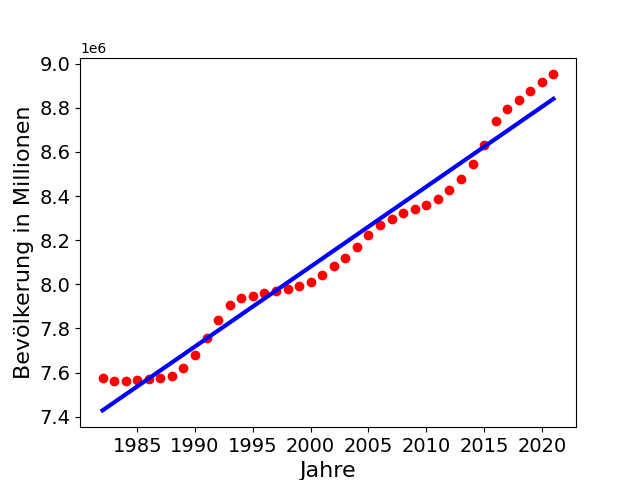
\includegraphics[width=0.6\textwidth]{images/population_linear.png}
\caption{Bevölkerungsentwicklung in Österreich}
\label{fig:pop_linear}
\vspace{-2.5cm}
\end{wrapfigure}

\noindent Die roten Punkte stellen die Ziel-\linebreak werte aus dem Datensatz dar. Die blaue Linie ist der Abbildung der Vorhersagen des Regressionsmodells. Die Visualisierung zeigt, dass das Modell das durchschnittliche Wachstum korrekt darstellt. Sie zeigt jedoch auch, das eine einfache lineare Regression keine genaue Vorhersage der Bevölkerung ermöglicht. Dafür ist eine andere Variante der Regression notwendig.

\vfill

\section{Visualisierung}
\label{sec:Visualisierung}

% Grundsätzliche Gründe für Visualisierung von Daten

Visualisierung stellt das Hauptthema dieser Bachelorarbeit dar. Einen guten Einstieg in dieses Thema bietet das Werk \emph{The visual display of quantitative information} \parencite{TufteEdward}. Demnach ist die Visualisierung ein Werkzeug zur Kommunikation von Daten. Die Stärke der Visualisierung ist es dabei, eine große Anzahl an Werten in einem kleineren Bereich darzustellen. Dadurch erleichtert die Visualisierung das Erkennen von Strukturen und Anomalien.\\
\noindent Diese Stärken sind im Vergleich der Abbildung  \ref{fig:visualization_advantage} zu sehen. Die Werte der Tabelle alleine sind nur schwer interpretierbar. Im Diagramm sind die Strukturen der beiden Klassen jedoch besser zu erkennen. Dort wird ersichtlich, dass sich die Punkte der beiden Klassen kaum überschneiden. Außerdem stechen in der Visualisierung die beiden Anomalien in den Daten heraus. Zwei Einträgen nähern sich dabei der jeweils anderen Klasse an. Die im Beispiel verwendeten Daten wurden mithilfe von Scikit-learn (Abschnitt \ref{sec:scikit-learn}) generiert.

\begin{figure}[H]
    \begin{minipage}{0.4\linewidth}
        \centering
        \begin{tabular}{ |c|c|c|c| } 
         \hline
           & X & Y & Klasse \\
          \hline
          0 & 1.771 & -1.54 & 1 \\
          1 & 4.346 & -7.57 & 1 \\
          2 & 5.737 & -9.69 & 1 \\
          3 & -1.07 & 1.486 & 0 \\
          4 & -1.37 & 1.528 & 0 \\
          5 & 1.342 & -8.97 & 1 \\
          6 & 1.417 & -9.93 & 1 \\
          7 & 1.336 & -1.34 & 1 \\
          8 & -5.78 & 2.561 & 0 \\
          9 & -1.21 & 1.173 & 0 \\
          \vdots & \vdots & \vdots & \vdots \\
          95 & -9.11 & 9.428 & 0 \\
          96 & -1.92 & 3.359 & 0 \\
          97 & -3.14 & 5.441 & 0 \\
          98 & 7.910 & -8.23 & 1 \\
          99 & -1.54 & 2.328 & 0 \\
         \hline
        \end{tabular}
    \end{minipage}
    \hfill
    \begin{minipage}{0.6\linewidth}
        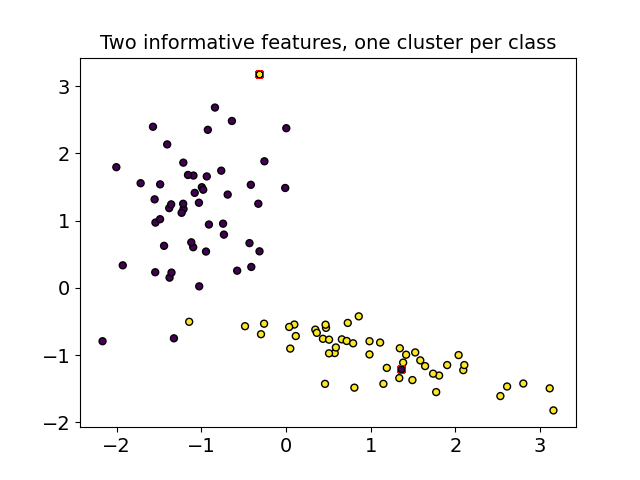
\includegraphics[width=1.1\linewidth]{images/visualization_advantage.png}
    \end{minipage}
    
    \caption{Beispiel zur Interpretation von Daten mittels Visualisierung}
    \label{fig:visualization_advantage}
\end{figure}

% Qualitätsmerkmale von Visualisierung und Warum sie wichtig sind
\noindent Für eine qualitative Visualisierung ist es wichtig die grafische Integrität einzuhalten. Laut Tufte wird dies durch das Einhalten von vier Regeln beschrieben:
\begin{enumerate}
    \item Konsistente Relation zwischen Größen in der Visualisierung und Zahlenwerten
    \item Konsistente Skalierung der Achsen
    \item Gleiche Anzahl an Dimensionen zwischen Visualisierung und Daten
    \item Darstellung aller für den Kontext relevanten Daten
\end{enumerate}

\noindent Diese Regeln wurden von Tufte in einem Zitat zusammengefasst: \emph{Show data variation, not design variation} \parencite{TufteEdward}. Das Brechen dieser Regeln, kann die Interpretation der dargestellten Daten beeinflussen.

% Aufgaben: Visualisierung
% - Beispiel für schlechte Umsetzung von Visualisierung / Visuelle Verzerrung


\section{Scikit-learn}
\label{sec:scikit-learn}

% Was ist scikit-learn?
Scikit-learn\footnote{https://scikit-learn.org/stable/index.html} \parencite{scikit-learn} ist eine Python-Bibliothek welche verschiedene Implementierungen von Machinelearning-Algorithmen bereitstellt. Ein Teil der Bibliothek stellt dabei verschiedene Implementierungen von Regression zur Verfügung. Ziel der\linebreak Bibliothek ist es, die Nutzung von Machinelearning-Algorithmen durch eine hohe Ebene der Abstraktion zu erleichtern. Zusätzlich bietet die Bibliothek eine gute Performance und eine umfassende Dokumentation der einzelnen Implementierungen. In der Praxis weist Scikit-learn eine weite Verbreitung vor. Das lässt sich aus den Statistiken der\linebreak Webseite \emph{libraries.io} feststellen\footnote{https://libraries.io/pypi/scikit-learn}. Dadurch ist die Unterstützung innerhalb von \linebreak Scikit-charts wichtig. Sie erlaubt es, dass Scikit-charts in vielen Projekten zur Anwendung kommen kann.\\\\
%Wie sieht die grundlegende API zur Verwendung aus?
\noindent Ein Überblick über die Schnittstellen der API ist in der Publikation \cite{sklearn_api} zu finden. Im Zentrum der Scikit-learn API befinden sich dabei drei Schnittstellen. Diese sind: \emph{estimator}, \emph{predictor} und \emph{transformer}.

\begin{itemize}
\item Der \emph{estimator} beschreibt ein Objekt, welches ein Modell aus Daten trainiert. Dafür wird eine \emph{fit} Methode definiert. Diese nimmt die Einflusswerte und optionale Zielwerte als Array an. Nach einem solchen Aufruf gilt das Modell als trainiert. Es kann nun für Vorhersagen und Analysen verwendet werden.
\item Der \emph{predictor} ist eine Erweiterung eines \emph{estimators}. Es beschreibt ein Objekt mit einer \emph{predict} Methode. Diese nimmt ein Array aus Einflusswerten entgegen und generiert daraus eine Vorhersage.
\item Der \emph{transformer} ist ebenfalls eine Erweiterung eines \emph{estimators}. Es beschreibt ein Objekt, welches Daten über eine \emph{transform}-Methode modifiziert oder filtert. Diese nimmt ein Array an und gibt die transformierte Version zurück.
\end{itemize}

\noindent Durch dieses flexible Design der API wird es ermöglicht, konkrete Implementierung auszutauschen. Dadurch wird es einfacher, allgemeine Algorithmen basierend auf diesen Modellen zu entwickeln. Im Rahmen dieser Arbeit ist besonders die \emph{predictor} Schnittstelle relevant. Diese bildet die Basis aller Regressionsmodell in Scikit-learn.

\section{Matplot}
\label{sec:matplot}

% Was ist Matplot und warum ist es interessant?
% Unterstützt 2D plots, 3D plots sowie interaktive Visualisierungen
% Hohe customizabilitie, viel einstellbar
% Wird in vielen Bibliotheken wie z.B. skicit-learn zur visualisierung verwendet
Bei Matplotlib \parencite{Matplot} handelt es sich um eine Python-Bibliothek zur Entwicklung von Visualisierungen. Die Bibliothek ermöglicht dabei sowohl 2D, 3D und\linebreak interaktive Visualisierungen. Die Visualisierungen können durch den Entwickler bis ins kleinste Detail konfiguriert werden. Dadurch werden auch komplexe Visualisierungen ermöglicht. Ein Beispiel dafür ist Abbildung \ref{fig:matplot_fig_anatomy}, welche mithilfe von Matplot generiert wurde. Die Abbildung dient ebenfalls als eine Übersicht über alle konfigurierbaren Elemente einer Visualisierung.

\begin{figure}[H]
\centering
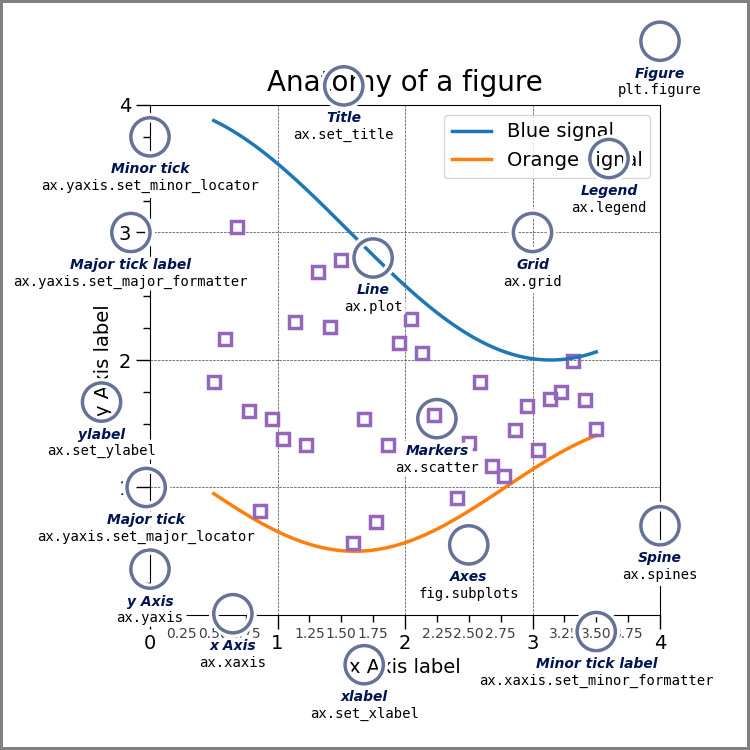
\includegraphics[width=.7\textwidth]{images/matplot_figure_anatomy.jpg}
\caption{Aufbau einer Matplotlib Visualisierung \protect\footnotemark}
\label{fig:matplot_fig_anatomy}
\end{figure}

\footnotetext{Quelle: https://matplotlib.org/3.7.1/gallery/showcase/anatomy.html}

% Wie sind die Klassen für das Rendering aufgebaut?
\noindent Basis einer Visualisierungen in Matplot sind laut API-Referenz\footnote{https://matplotlib.org/3.7.1/api/index.html} zwei Klassen: \emph{Figure} und \emph{Axes}. Eine \emph{Figure} beinhaltet alle Daten und Objekte einer Visualisierung. Diese kann einen übergreifende Titel, Legende, mehrere \emph{Axes} sowie \emph{Sub-Figures} beinhalten.\\
\noindent Eine \emph{Axes} beschreibt Bereiche einer \emph{Figure}, in welchen Daten dargestellt werden. Diese Objekte verwalten die einzelnen Linien, Datenpunkte sowie Achsenkonfigurationen. In der Abbildung \ref{fig:matplot_fig_anatomy} betrifft das alle hervorgehobenen Elemente, welche mit \emph{ax.} beginnen.\\\\
% Arten der Anwendung der API?
\noindent Die Anwendung der Matplot-API kann entweder explizit oder implizit erfolgen. Bei der expliziten Anwendung werden \emph{Figure}- und \emph{Axes}-Objekte direkt erstellt und verwaltet. Es handelt sich dabei um einen objektorientierten Ansatz. Bei der impliziten Anwendung wird die \emph{matplotlib.pyplot} API verwendet. Es handelt sich dabei um einen state-basierten Ansatz, bei welchem die Objekte von der API verwaltet werden. Für diese Arbeit wird rein die explizite Anwendung verwendet, um eine genaue Kontrolle über die Visualisierungen zu behalten.\\\\
% wo ist rendering unterstützt?
\noindent Um unterschiedliche Anwendungsfälle zu ermöglichen, unterstützt Matplot eine Reihe an \emph{Back-Ends} für die Darstellung. Nicht-interaktive Back-Ends werden zum Speichern von Visualisierungen verwendet (z.B. PNG, PDF, ...). Interaktive Back-Ends\linebreak unterstützen verschiedene betriebssystemunabhängige UI-Systeme, sowie einen Web-Server und \nameref{sec:jupyter_notebook}. Für diese Arbeit ist es dementsprechend notwendig zu Testen, ob die Diagramme auf den unterstützten \emph{Back-Ends} funktionieren. Gefundene Einschränkungen müssen ebenfalls hervorgehoben werden.

\section{Jupyter Notebook}
\label{sec:jupyter_notebook}

Jupyter Notebooks \parencite{kluyver2016JupyterN} sind ein Datenformat zum Austausch von Code-Ausschnitten und Beschreibungen. Über eine eigene Laufzeitumgebung\footnote{https://jupyter.org/} können die Notebooks interaktiv im Browser ausgeführt werden. Sie sind werden oft im\linebreak wissenschaftlichen Umfeld verwendet, um Ergebnisse auszutauschen. Sie besitzen ebenfalls eine Unterstützung der Programmiersprache Python. Für Scikit-charts ist es dementsprechend notwendig, Jupyter Notebooks zu unterstützen.

\section{ROC- / REC-Kurven}
\label{sec:roc_rec}

ROC und REC Kurven werden in einigen Bibliotheken zur Visualisierung von Regressionsmodellen angeboten. \emph{Receiver Operating Characteristic} (ROC) Kurven werden Verwendet, um die Qualität von Klassifizierungsfunktionen zu bewerten. Auf der Y-Achse wird dabei der Prozentsatz der echt positiven Werte aufgetragen. Auf der X-Achse wird der Prozentsatz der falsch positiven Werte aufgetragen. Die Performance wird bei ROC-Kurven in dem Bereich unter der Kurve (AUC) beschrieben. Diese ist bei zufälligen Funktionen etwa 0.5 und bei Funktionen mit immer richtigen Ergebnissen 1. Dieses Prinzip kann auch zum Vergleich zweier beliebiger Funktionen über ihre Ergebnisse angewandt werden.

\begin{wrapfigure}{l}{0.55\textwidth}
\vspace{-1cm}
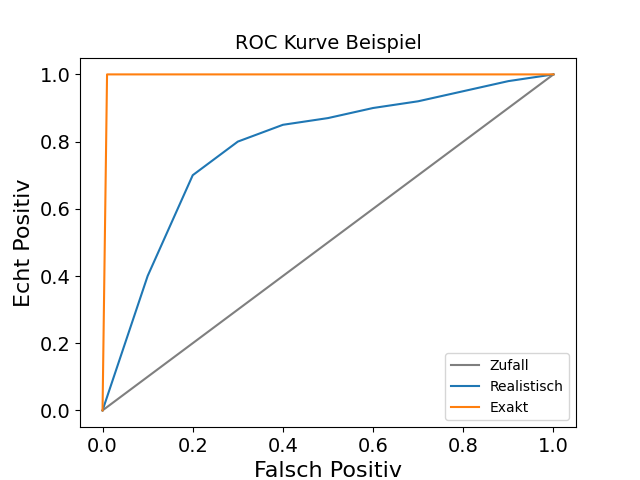
\includegraphics[width=0.6\textwidth]{images/roc_example.png}
\caption{Beispiel für ROC-Kurven}
\label{fig:roc_example}
\vspace{-4cm}
\end{wrapfigure}

\noindent Die \emph{Regression Error Characteristic} (REC) Kurve ist eine Anwendung des Prinzips von ROC für Regression. Im Gegensatz zur ROC-Kurve wird hier auf der X-Achse der absolute Unterschied zwischen Vorhersage und Zielwert dargestellt.\linebreak \parencite{RocRec}

\vspace{3.5cm}

\pagebreak

\section{Pandas}
\label{sec:pandas}

% Was ist es?
% Wie / wofür wird es verwwendet?
Pandas \parencite{pandas} ist eine Python-Bibliothek zur Verwaltung und Analyse von tabellarischen Daten. Sie wird in der Bibliothek zur Verwaltung der Diagrammdaten, sowie dem Laden des Beispieldatensatzes verwendet. Den Kern der\linebreak Bibliothek stellt die \emph{Dataframe} Datenstruktur. Diese verwaltet die Daten als eine\linebreak Tabelle. Der Zugriff auf die Daten ist beliebig über die Spaltennamen oder Zeilen-Indices möglich. Ein Zugriff kann ebenfalls mithilfe von Pythons \emph{Slicing}\footnote{https://docs.python.org/3/reference/expressions.html\#slicings} erfolgen. Dadurch ist es möglich, einzelne Teilbereiche als eigenen Dataframe auszuwählen.\\\\
\noindent Neben dem intuitiven Zugriff vereinfacht die Bibliothek das Serialisieren und Deserialisieren von Datensätzen. Dafür werden \emph{read\_} und \emph{write\_} Funktionen zur Verfügung\linebreak gestellt. Diese Unterstützen verschiedene Datenformate wie CSV, Excel, SQL oder JSON. Die Datenstruktur bietet außerdem eingebaute Funktionen zur Analyse der\linebreak Daten. Mithilfe dieser können beispielsweise Median, Durchschnittswert sowie Mininum und Maximum ausgewählt werden. Außerdem gibt es eine eingebaute Visualisierung der Daten mithilfe von Matplotlib. Beispielsweise können Histogramme, Boxplots oder Streudiagramme über die Daten generiert werden.



\section{Partial dependence}
\label{sec:partial_dependence}

Mithilfe der \emph{partial dependence}, zu deutsch \emph{partielle Abhängigkeit}, kann der relative Einfluss von Variablen auf eine Funktion beschrieben werden. Die partial dependence wird deshalb für die Darstellung des Schnittdiagramms benötigt. Wie dieser Wert berechnet wird ist in dem Buch "The Elements of
Statistical Learning" \parencite{elements_statistical_learning}\linebreak beschrieben.\\\\
\noindent Darin werden zwei Mengen $X_S$ und $X_C$ definiert. $X_S$ beschreibt die Einflussvariablen, für welche die partial dependence berechnet wird. $X_C$ beschreibt die restlichen Einflussvariablen. Das Ergebnis der Funktion $f(X)$ ergibt sich dementsprechend aus $f(X) = f(X_S, X_C)$. Das Ergebnis der Funktion für konkrete Werte von $X_S$ kann\linebreak somit durch den Erwartungswert über alle Werte von $X_C$ beschrieben werden. In der Bibliothek kann dies über die konkreten Werte $x_C$ im Datensatz angenähert werden.

\begin{equation}
  \begin{aligned}
    \bar{f}_S(X_S) = \frac{1}{N}\sum_{i=1}^{N}f(X_S, x_{iC})
  \end{aligned}
  \label{fig:partial_dependence}
\end{equation}

\noindent Der Wert $N$ entspricht dabei der Anzahl an Einträgen im Datensatz. Der Einfluss der Variablen $Xs$ wird beschrieben über die Relation zwischen den eingesetzten Werten sowie den Ergebnissen $\bar{f}_S(X_S)$.

%   - Partial-Dependency-Plot
%       - https://slds-lmu.github.io/iml_methods_limitations/pdp.html
%       - https://www.tandfonline.com/doi/full/10.1080/10618600.2014.907095
%       - https://en.wikipedia.org/wiki/Partial_derivative
%       - https://hastie.su.domains/ElemStatLearn/printings/ESLII_print12_toc.pdf Seite 388
\chapter{Metriken und Diagramme}
\label{cha:Metriken_Diagramme}

% Idee: Hervorheben wofür die Diagramm genutzt werden? Feature-Importance, ...

Dieses Kapitel beschäftigt sich mit der Analyse der einzelnen Diagrammtypen und\linebreak ihrer Implementierung in HeuristicLab \parencite{HeuristicLab}.
Hierbei wird zuerst untersucht welche Informationen in den Diagrammen visualisiert werden. Danach\linebreak erfolgt eine genaue Analyse jedes Diagrammtyps.
Das Ziel ist es herauszufinden, welche Informationen durch die Visualisierung gewonnen werden. Außerdem werden die Funktionalitäten der einzelnen Diagramme definiert. 
Diese dienen als Anforderungen an die Implementierung in Scikit-charts. Im weiteren Schritt werden diese Informationen\linebreak verwendet, um bestehende Bibliotheken mit HeuristicLab zu vergleichen.

\section{Metriken}
\label{cha:Metriken}

Die Metriken in HeuristicLab werden aus den Einträgen des Datensatzes und den\linebreak Vorhersagen gesammelt. Folgende Metriken können aus den einzelnen Diagrammen\linebreak erkannt werden:

\begin{description}
\item[Index] \hfill\newline
Die Position des Eintrages im Datensatz.
\item[Zielwert] \hfill\newline
Der beobachtete Wert der Zielvariable im Datensatz.
\item[Vorhersage] \hfill\newline
Der berechnete Wert des Regressionsmodells für die gegebenen Einflussvariablen.
\item[Residuum] \hfill\newline
Der Unterschied von Zielwert und Vorhersage (\cite{RegressionGrundlagen}).
\item[Relativer Fehler]  \hfill\newline
Das Residuum relativ zum Zielwert.
\item[Einflussvariablen] \hfill\newline %Features
Die Werte der Variablen im Datensatz, aus welchen das Regressionsmodell die Vorhersage berechnet. Im Englischen auch \textit{Feature} genannt.
\end{description}

\vspace{\baselineskip}

\noindent Residuum und Fehler haben außerdem einen zusätzlichen zweiten Eintrag, mit absoluten Zahlenwerten.

\section{Allgemeine Funktionen der Diagramme}
\label{sec:allgemeine_funktionen_diagramme}

Alle Diagramme, außer dem Schnittdiagramm, unterstützen ein Zoomen mithilfe der Maus. Dabei kann ein Bereich des Diagramms ausgewählt werden, um ihn über die gesamte Größe anzuzeigen. Durch einen Doppelklick mit der linken Maustaste wird der Bereich wieder zurückgesetzt.

%ToDo: Beschreibung der Informationen welche daraus gewonnen werden!

\section{Liniendiagramm (line chart)}
\label{sec:line-chart}

Das Liniendiagramm vereinfacht das Erkennen von Mustern im Verlauf der Daten. Durch den Vergleich von Zielwerten und Vorhersagen kann außerdem geprüft werden, ob sich dieser Verlauf im Modell widerspiegelt. Dadurch bietet sich das Diagramm für Datensätze mit gereihten Daten an.

\begin{figure}[H]
    \centering
    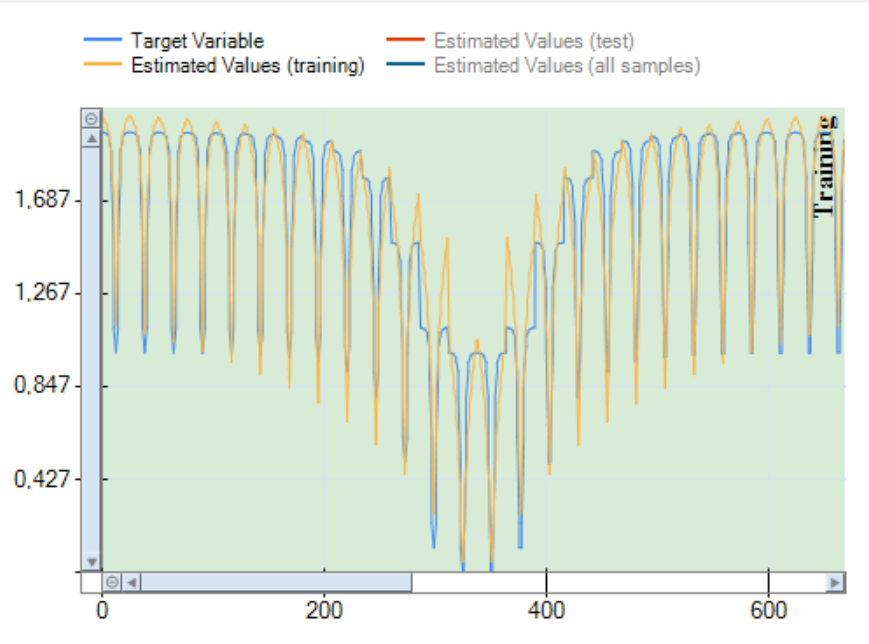
\includegraphics[height=.6\textwidth]{images/line-chart_small.png}
    \caption{Liniendiagramm in HeuristicLab}
    \label{fig:example_line_chart}
\end{figure}

\noindent Die Y-Achse gibt den Wertebereich der Zielvariable und der Prognosen an. Auf der\linebreak X-Achse ist der aufsteigende Index der Einträge angegeben.
Danach werden die Zielwerte und Vorhersagen als Punkte eingetragen und verbunden. Durch den Klick auf dem jeweiligen Namen kann die Anzeige der Werte aktiviert und deaktiviert werden.

\pagebreak

\section{Streudiagramm (scatter plot)}
\label{sec:scatter-plot}

Wie das Liniendiagramm dient auch das Streudiagramm zum Vergleich von Zielwerten und Vorhersagen. Die Reihenfolge der Beobachtungen im Datensatz, werden jedoch in diesem Diagramm ignoriert. Das Streudiagramm wird genutzt um zu prüfen,
ob es systematische Fehler in der Vorhersage der Werte gibt. Ist das nicht der Fall, sollten sich die Punkte der Geraden im Diagramm annähern.

\begin{figure}[H]
    \centering
    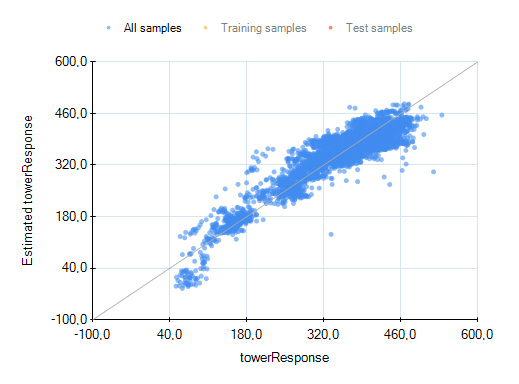
\includegraphics[height=.6\textwidth]{images/scatter-plot.png}
    \caption{Streudiagramm in HeuristicLab}
    \label{fig:example_scatter_plot}
\end{figure}

\noindent Die Y-Achse gibt den Bereich der Vorhersagen an. Auf der X-Achse sind die Zielwerte angegeben. Jeder eingetragene Punkt im Diagramm beschreibt die Überschneidung\linebreak dieser Werte. Die durchgehende Linie zeigt den Bereich an, auf welchem beide Achsenwerte ident sind.

\pagebreak

\section{Blasendiagramm (bubble chart)}
\label{sec:bubble-chart}

Das Blasendiagramm dient zur interaktiven Analyse der Zusammenhänge aller Variablen.
Er bietet sich also ebenfalls sehr gut an, um Fehler im Modell zu prüfen. Die dynamischen Interaktionen vereinfachen dabei die Analyse.

\begin{figure}[H]
    \centering
    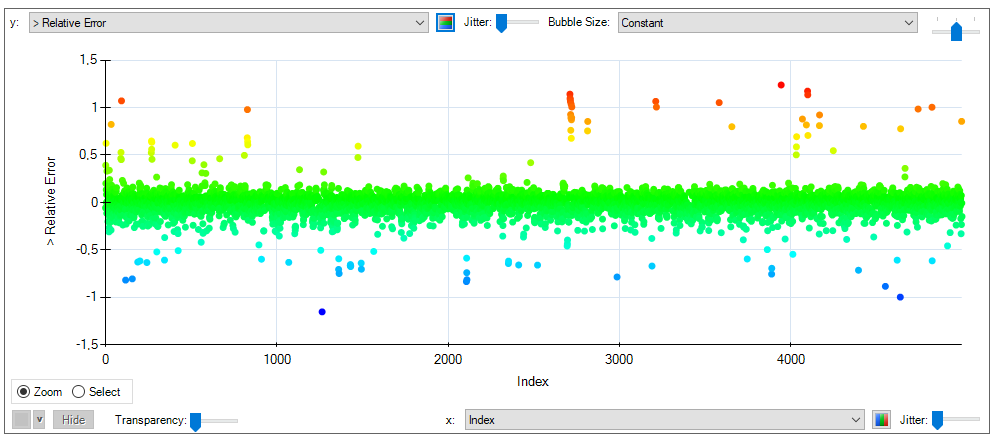
\includegraphics[height=.5\textwidth]{images/bubble-chart.png}
    \caption{Blasendiagramm in HeuristicLab}
    \label{fig:example_bubble_chart}
\end{figure}

\noindent Jede der aufgezeichneten Blasen zeigt einen einzelnen Eintrag im Datensatz. Die Variablen auf beiden Achsen können frei gewählt werden. 
Es ist ebenfalls möglich, einzelne Einflussvariablen auszuwählen.\newline\newline
Die Farben der Blasen können dynamisch gesetzt werden. Der Knopf neben der Metrik-auswahl setzt die Farben automatisch nach dem
Verlauf der Achse. In der Abbildung \ref{fig:example_bubble_chart} ist diese Färbung für die Y-Achse zu sehen. Außerdem ist es möglich, einen\linebreak Bereich von Blasen auszuwählen. Dieser kann danach explizit zu gefärbt oder ausgeblendet werden. Die Blasen behalten ihre Farbeinstellungen beim Wechseln der Metriken.\newline\newline
Die Jitter-Option neben der Metrikauswahl ermöglicht es, einen Versatz der gezeichneten Blasen einzustellen. Diese Option ist in beide Achsenrichtungen möglich.
Die Größe der einzelnen Blasen kann ebenfalls verändert werden. Die Option dafür ist in der rechten oberen Ecke zu finden. Der Wert der Größe kann konstant oder relativ zu einzelnen Metriken gesetzt werden. Zuletzt besteht ebenfalls die Option, die Transparenz der Blasen zu verändern.

\pagebreak

\section{Schnittdiagramm (partial dependency plot)}
\label{sec:partial-dependency-plot}

Das Schnittdiagramm dient zur Analyse der Zusammenhänge zwischen den Einflussvariablen und den Vorhersagen, die im Modell erfasst sind. Dadurch kann die Art der Abhängigkeit von Variablen als Funktion dargestellt werden. Diese Informationen\linebreak können für die Validierung und Plausibilisierung von Modellen helfen.

\begin{figure}[H]
    \centering
    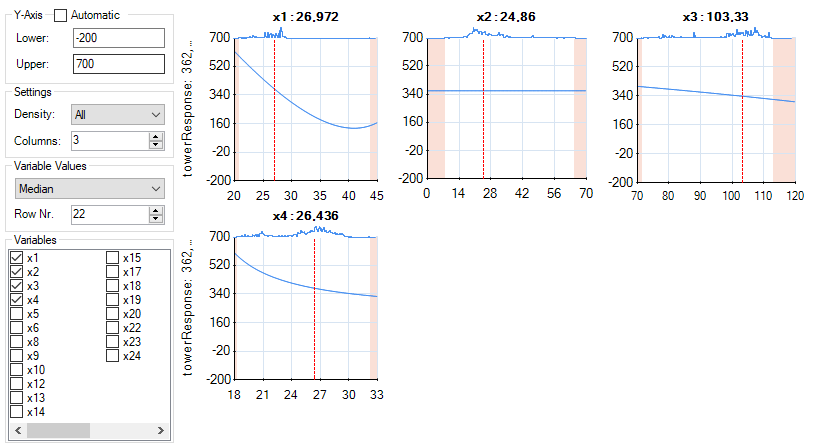
\includegraphics[height=.5\textwidth]{images/intersection-plot.png}
    \caption{Schnittdiagramm in HeuristicLab}
    \label{fig:example_partial_dependency_plot}
\end{figure}

\noindent Im rechten Bereich werden die Teildiagramme für die einzelnen Einflussvariablen abgebildet. Auf der Y-Achse werden die Vorhersagen dargestellt.
Die X-Achse repräsentiert die möglichen Werte der einzelnen Variablen. Die rot hinterlegten Bereiche befinden sich nicht im Datensatz,
sondern normalisieren den Wertebereich der Achse.
Die blaue Linie ist der Verlauf des Zusammenhangs zwischen Vorhersage und Variablenwert.\newline\newline
Der Text zu Beginn der Zeilen gibt den Wert der aktuellen Vorhersage an.
Im Titel steht der Name der Variable sowie ihr aktueller Wert. Dieser ist ebenfalls im Diagramm durch die rote Linie markiert. 
Diese Linie kann mit dem Mauszeiger verschoben werden. Dadurch werden sowohl Variablenwert, als auch die Vorhersage aktualisiert.
Die blaue Linie, oben an den Diagrammen, beschreibt die Dichte des Datensatzes über die X-Achse.\newline\newline
Im linke Bereich befinden sich Optionen um die Darstellung der Teildiagramme zu verändern. Dabei handelt es sich um den Wertebereich der Y-Achse und die Anzahl der Spalten im rechten Bereich. Außerdem kann der initiale Wert der Variablen in den Teildiagrammen gesetzt werden. Mögliche Werte sind der Median, der Durchschnittswert sowie bestimmte Zeilen im Datensatz. Die Diagramme können für einzelne Variablen aktiviert und deaktiviert werden.
\chapter{Existierende Bibliotheken}
\label{cha:existirende_bibliotheken}

Bestehende Bibliotheken bieten eigene Visualisierungen von Regressionsmodellen an. In diesem Kapitel werden einige davon analysiert und mit den Anforderungen der Ziel-setzungen \ref{sec:Zielsetzung} und den Funktionen der Diagramme in Kapitel \ref{cha:Metriken_Diagramme} verglichen. Das Ziel ist es herauszufinden, welche Visualisierungen und Funktionalitäten bereits von bestehenden Bibliotheken abgedeckt werden.

\section{SlickML}
\label{sec:SlickML}
SlickML \parencite{slickml2020} ist eine Python-Bibliothek zur Entwicklung von Machinelearning-Modellen. Als Ziel setzt sich die Bibliothek "eine schnelle Experimentierung mit Modellen und maximale Ableitung von Informationen". Die Bibliothek\linebreak befindet sich noch in Entwicklung, bietet jedoch einzelne Funktionen zum Trainieren von Modellen, Hyperparameter-Optimierung sowie Sammlung und Visualisierung von Metriken.\\\\
\noindent Für Regressionsmodelle gibt es eine Funktion, welche Metriken aus Zielwerten sowie Vorhersage sammelt und visualisiert. Die generierten Diagramme und gewählten Metriken können dabei nicht beeinflusst werden. Bei den dargestellten Metriken handelt es sich um die Vorhersage relativ zu den Zielwerten, die Frequenz einzelner Vorhersagen, verschiedene Auswertungen vom Residuum, sowie der REC-Kurve (Abschnitt \ref{sec:roc_rec}).

%https://github.com/slickml/slick-ml
%https://docs.slickml.com/pages/quick_start.html
%https://www.docs.slickml.com/autoapi/slickml/metrics/index.html#slickml.metrics.RegressionMetrics

\section{Seaborn}
\label{sec:seaborn}

Seaborn \parencite{seaborn} ist eine Python-Bibliothek für Datenvisualisierung, welche auf Matplot aufbaut. Die Bibliothek stellt die API von Matplot auf einer höheren Ebene zur Verfügung. Anwender:innen wird dadurch ermöglicht, einfach attraktive Visualisierungen von Datensätzen zu erstellen.\\\\
\noindent Die Bibliothek unterstützt eine Vielzahl an implementierten Diagrammen. Diese können mithilfe eines einzelnen Aufrufs zur Visualisierung von Datensätzen verwendet werden. Jedes dieser Diagramme kann mithilfe von visuellen Themen und einem eigenen Objekt-Interface weiter angepasst werden. Außerdem ist es möglich, mehrere Diagramme zu einer gemeinsamen, komplexeren Visualisierung zusammenzufügen. Ein Beispiel dafür ist in Abbildung \ref{fig:example_seaborn} zu sehen. Seaborn besitzt jedoch keine explizite Unterstützung für interaktive Diagramme.

\begin{figure}[H]
    \centering
    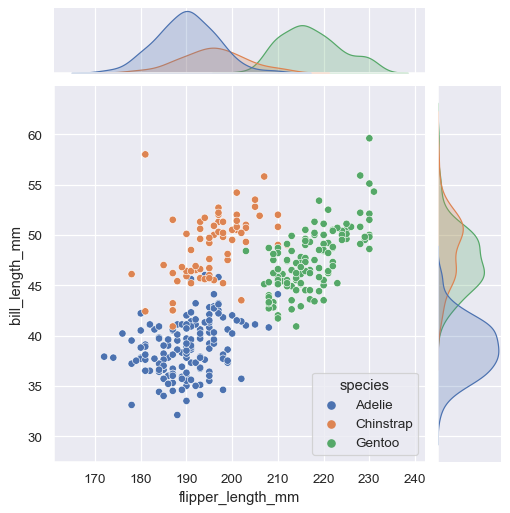
\includegraphics[height=.6\textwidth]{images/seaborn_example.png}
    \caption{Beispiel eines Streudiagramms mit Randverteilung in Seaborn\protect\footnotemark}
    \label{fig:example_seaborn}
\end{figure}

\footnotetext{Quelle: https://seaborn.pydata.org/tutorial/introduction.html}

% https://joss.theoj.org/papers/10.21105/joss.03021
% https://seaborn.pydata.org/
% https://seaborn.pydata.org/tutorial/function_overview.html#similar-functions-for-similar-tasks
% https://seaborn.pydata.org/tutorial/regression.html?highlight=regression
% https://seaborn.pydata.org/examples/index.html


\section{Plotly}
\label{sec:plotly}

Plotly\footnote{https://github.com/plotly/plotly.py} ist eine Bibliothek für interaktive Visualisierung, mit Unterstützung von Python. Sie besitzt ebenfalls Implementierungen für R, Julia, Javascript, sowie andere Sprachen. Die Bibliothek ermöglicht verschieden 2D- und 3D-Diagramme, sowie Visualisierungen für Karten.\\\\
\noindent Alle Diagramme besitzen automatisch eine Zoom-Funktion, Tooltips sowie die\linebreak Möglichkeit den Bildbereich zu verschieben. Die Visualisierungen können sowohl\linebreak Lokal, im Web und auch in Jupyter-Notebook dargestellt werden. Neben einer Vielzahl\linebreak anderer Diagramme werden auch Liniendiagramm, Streudiagramm und Blasendiagramm\linebreak unterstützt. Die zusätzliche Interaktivität beschränkt sich hier jedoch auf das Ein- und Ausblenden von Datenklassen. Zusätzliche Funktionen wie eine dynamische Wahl der Metriken können jedoch eigenständig implementiert werden. Dafür bietet die\linebreak Bibliothek Unterstützung für UI-Elemente wie Knöpfe und Drop-Down-Elemente.\linebreak Dementsprechend konkurriert diese Bibliothek hauptsächlich mit Matplot.

\begin{figure}[H]
    \centering
    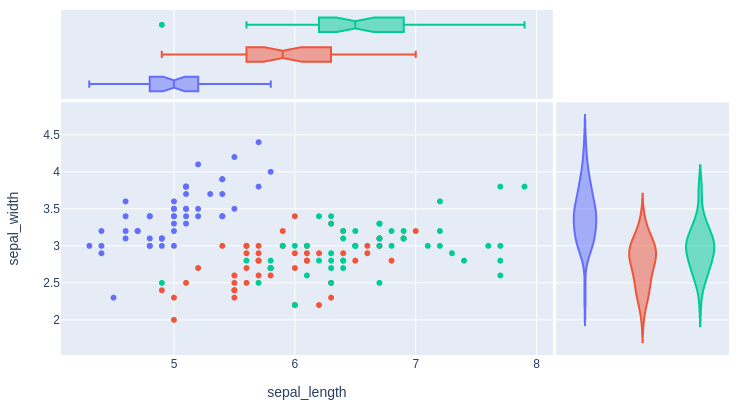
\includegraphics[height=.6\textwidth]{images/plotly_example.png}
    \caption{Beispiel eines Streudiagramms mit Randverteilung in plotly\protect\footnotemark}
    \label{fig:example_plotly}
\end{figure}

\footnotetext{Quelle: https://plotly.com/python/marginal-plots/}

% https://github.com/plotly/plotly.py
% https://plotly.com/python/
% https://plotly.com/python/ml-regression/

\section{Ergebnis}

Es gibt aktuell eine gute Auswahl an Bibliotheken welche, sich mit dem Thema Visualisierung beschäftigen. Wie in der Problemstellung angemerkt, schafft es jedoch keine den Anforderungen von Scikit-charts genau zu entsprechen.\\
\begin{itemize}
    \item Die Visualisierung in SlickML ist statisch und zu spezifisch. 
    \item Seaborn bietet eine gute Erweiterung von Matplot an. Die Bibliothek ist außerdem einfach zu verwenden. Sie bietet jedoch keine erweiterte Unterstützung von dynamischen Interaktionen.
    \item Plotly bietet dynamische Visualisierungen und eine gute Integration in Jupyter Notebooks, sowie Webseiten. Der Umfang der Funktionen entspricht jedoch nicht dem Umfang, welcher in dem Kapitel \ref{cha:Metriken_Diagramme} identifiziert wurden.
\end{itemize}

\vspace{\baselineskip}

\noindent Alle diese Bibliotheken besitzen dementsprechend Einschränkungen bezüglich der\linebreak Aufgabenstellung. Trotzdem bieten Sie eine gute Basis um Visualisierungen in ein\linebreak Projekt einzubauen. Die Bibliothek dienen außerdem als eine Inspiration für die\linebreak Implementierung von Scikit-charts.

% Referenz auf Problemstellung -> Zu einfach und Statisch, erneut aufwand notwendig, inflexibel. Keine komplette Abdeckung der Zielsetzung jedoch
\chapter{Design der Bibliothek}
\label{cha:design_der_bibliothek}

Diese Kapitel beschäftigt sich mit dem Design der Bibliothek, welche im Zuge dieser Arbeit erstellt wurde. Zuerst werden die Abhängigkeiten zu anderen Bibliotheken  \linebreak beschrieben und für diese argumentiert. Danach wird auf die Architektur der Bibliothek eingegangen. Die Sammlung und Berechnung von Metriken wird beschrieben. Zuletzt wird noch das Design der Diagramm-Komponenten erläutert.


\section{Abhängigkeiten auf andere Bibliotheken}
\label{sec:base_library}

% Gewählte Technologien zur Umsetzung
%   - maptlot
%   - numpy
Scikit-charts wird basierend auf Matplot, Numpy, Pandas und Scikit-learn entwickelt. Dabei wird bei den Versionsnummern grundsätzlich von der neuesten Version ausgegangen. Als Alternative zu Matplot wurde kurzzeitig Seaborn in Erwägung gezogen. Die zusätzliche Unterstützung für angehängte Diagramme an den Achsen würde die Implementierung des Schnittdiagramms vereinfachen. Das alleine rechtfertigt jedoch nicht die Abhängigkeit zur Bibliothek.\\\\
\noindent Numpy \footnote{https://numpy.org/} wird in der Bibliothek zur optimierten Berechnung der Metriken benötigt. Es handelt sich dabei um den De-facto-Standard zum effizienten Rechnen von N-dimensionalen Arrays in Python. Numpy-Arrays bieten außerdem weiter Funktionen um die Verwendung von Arrays zu vereinfachen. Grundlegende Arithmetische Funktionen können\linebreak direkt auf Numpy-Arrays angewandt werden. Zusätzlich werden verschiedene statistische Funktionen zur Auswertung angeboten.\\\\
\noindent Die Pandas-Bibliothek bietet eine Datenstruktur sowie Funktionen zur Verwaltung von tabellarischen Daten. Diese wird zentral bei der Berechnung und Verwaltung der\linebreak Metriken verwendet.\\\\
\noindent Scikit-learn wird in der Bibliothek nur zur Berechnung der \emph{partial dependence}\footnote{https://scikit-learn.org/stable/modules/partial\_dependence.html\#partial-dependence-plots} (Abschnitt \ref{fig:partial_dependence}) aus einem Modell benötigt. Dadurch ist das Schnittdiagramm als einziges auf Scikit-learn Modelle beschränkt. Sonstige Diagramme sind von Scikit-learn unabhängig. In diesen wird nur ausgegangen, dass die verwendeten Objekten der formellen Definition laut Dokumentation entspricht. Durch diesen Ansatz kann die Bibliothek auch mit anderen Implementierungen von Regressionsmodellen verwendet werden.\\\\
\noindent Zuletzt wird noch eine Abhängigkeit Pytest\footnote{https://docs.pytest.org/en/7.4.x/} benötigt. Diese Bibliothek wird für die Entwicklung von Tests in der Bibliothek verwendet.

\section{Sammeln von Metriken aus Modellen}
\label{sec:design_sammeln_metriken}

Das Sammeln der Metriken aus einem Modell soll mithilfe eines einzelnen Funktionsaufrufs möglich sein. Für die Berechnung werden zwei Werte benötigt. Zum Einen eine Referenz auf die \emph{predict}-Funktion eines \emph{predictors} (Abschnitt \ref{sec:scikit-learn}). Zum Anderen der originale Datensatz, aus welchem das Modell erstellt wurde.  Wie in Scikit-learn wird dieser als X- und Y-Arrays übergeben. Das Ergebnis wird als ein Pandas-Dataframe\linebreak zurückgegeben. Dieser enthält alle Metriken, welche zur finalen Visualisierung notwendig sind.

\begin{PythonCode}
PredictFunction: TypeAlias = Callable[[Tuple[float]], float]

def create_metrics(
        x: Union[np.ndarray[float], list[list[float]]],
        y: Union[np.ndarray[float], list[float]],
        predict: PredictFunction
) -> DataFrame:
\end{PythonCode}

% Wie werden die gesammelten Daten verwaltet?
%   - Pandas-Dataframe verwenden und als Argument zurückgeben (Argumentieren warum)
% Warum?
%   - Direkter Zugriff auf gesammte Metrik / einzelne Werte
%   - Flexibel -> Hinzufügen / Entfernen von Metriken
%   - Einfache erstellung berechneter Spalten
%   - Existierende Funktionen zum Filtern + Sortieren der Werte
\noindent Ein DataFrame bietet einige Vorteile gegenüber einer eigens implementierten Datenstruktur. Sie unterstützt einen indizierten Zugriff. Damit können sowohl einzelne Einträge als auch alle Werte einer Metrik ausgewählt werden. Weiters ist die Datenstruktur flexibel. Sie kann noch nach der Erstellung um Spalten erweitert werden. Die Erstellung von berechneten Spalten aus anderen Metriken wird ebenfalls unterstützt. Außerdem existieren bereits Funktionen zum Filtern und Sortieren der Daten.\\\\

%   - Argumentation: Nutzung von Funktionsreferenz +  Beschreibung von X / Y
\noindent Wie bereits angemerkt wird durch die Übergabe einer einzelnen \emph{predict}-Funktion die Flexibilität der Berechnung erhöht. Typinformationen aus Scikit-learn werden nicht benötigt. Es werden außerdem beliebige Modelle anderer Bibliotheken unterstützt. Möglicherweise inkompatible Funktionen können dabei über eigene Lambda-Funktionen an das Interface angepasst werden. Durch dieses Design wird ebenfalls die Testbarkeit der Funktion erleichtert. Bei einer Abhängigkeit auf ein Scikit-learn Modell würde ein\linebreak eigenes Mocking-Framework benötigt werden.\\\\

% Metriken welche gesammelt werden?
%       - Metriken aus Kapitel über Heuristiclab
%       - Accuracy pro Wert ausrechnen für REC-Nachstellung
%           - https://scikit-learn.org/stable/modules/model_evaluation.html#roc-auc-binary
%       - Deviation für REC Kurve
\noindent Die zurückgegebenen Metriken im Dataframe entsprechen den Metriken im Abschnitt \ref{sec:design_sammeln_metriken}. Die Berechnung der einzelnen Metriken, sowie deren Namen für den Spaltenzugriff sind nachfolgend aufgelistet.

\pagebreak

% Wie werden die Metriken berechnet?
\begin{description}
\item[index] \emph{i}\hfill\newline
\emph{i} entspricht dem aktuellen Index einer Zeile im Datensatz.
\item[x0 ... xn] \emph{x[i][n]}\hfill\newline
\emph{x} entspricht den Werten der Einflussvariablen für die predict-Funktion.\newline \emph{n} entspricht dem Index einer Einflussvariable.
\item[target] \emph{y[i]}\hfill\newline
\emph{y} entspricht den Zielwerten aus dem Datensatz.
\item[prediction] \emph{predict(x[i])} \hfill\newline
\emph{prediction} entspricht Funktion eines Modells, welche für Werte der Einflussvariablen eine Vorhersage generiert.
\item[residual] \emph{target - prediction}\hfill
\item[relative\_error] \emph{residual / target}\hfill
\end{description}

\section{Aufbau der Diagramme}
\label{sec:design_aufbau_diagramme}
% Wie werden einzelne Diagramme umgesetzt aus Metriken (Allgemein)?

% Allgemeiner Aufbau + Features dieser Klassen / Funktionen 
%       - Basisklasse für Implementerierung + Funktion für erstellung aus Daten & Predict
%       - Zurückgeben von Plot-Objekt damit user anpassen kann (Labels, ...)
Jedes der Diagramme besitzt den selben Aufbau. Es existiert eine Klasse, welche die Funktionalitäten des Diagramm implementiert. Die Klasse dient dabei sowohl zur Strukturierung des Codes, als auch zum Halten aller benötigten Referenzen an einem Ort. Eine weitere Funktion mit dem Namen des Diagramms dient zur Instanziierung der Klasse. Die übergebenen Argumente werden darin für die Klasse vorbereitet und an den Konstruktor übergeben. Zurückgegeben wird am Ende nur das eigentliche Figure-Objekt. Die konkrete Implementierung der Diagramme bleibt dadurch für die Benutzer:innen der Bibliothek verborgen. Über das zurückgegebene Figure-Objekt kann das Diagramm angezeigt werden. Mithilfe von Matplot lassen sich außerdem weitere visuelle Anpassungen über das Figure-Objekt am Diagramm vornehmen.

\begin{figure}[H]
    \centering
    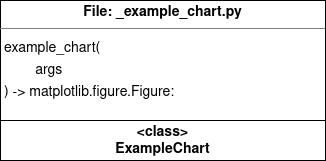
\includegraphics[width=0.4\textwidth]{images/uml_chart_design.png}
    \caption{Grundlegende Struktur einer Diagramm-Implementierung}
    \label{fig:uml_chart_design}
\end{figure}

%       - Compositions-Basiert (Allgemeine Fuhktionen wie Zoom select, etc) + Warum keine Vererbung?
\noindent Um gemeinsame Funktionalitäten zwischen den Diagrammen zu teilen wird mit Komposition gearbeitet. Funktionalitäten wie UI-Elemente werden dabei als eine unabhängige Komponente implementiert. In den Diagrammklassen selbst werden diese Komponenten dann angewandt. Vererbung wurde hierbei nicht gewählt, wegen den großen funktionalen Unterschieden zwischen den Diagrammen. Die Implementierung der Hilfsfunktionen und Klassen erfolgt dabei je nach Bedarf.
\chapter{Implementierung}
\label{cha:implementierung}

Dieses Kapitel bietet einen Überblick über die Implementierung der Bibliothek. Dabei werden einige Stellen aus dem Quellcode vorgestellt und ihre Funktionalität näher beschrieben. Dieses Kapitel enthält ebenfalls Durchführung und Beschreibung entwickelten Testfälle.

\section{Strukturierung und Typisierung in Python}
\label{sec:impl_structure_problems}

% - Module aufgeteilt in mehrere Dateien -> Was exportiert wird in __init__.py des Ordners definiert
Zu Beginn der Implementierung wurde die grundlegende Struktur des Codes festgelegt. Die Code-Basis der Bibliothek ist auf zwei Python-Module aufgeteilt: \emph{scikit\_charts} und \emph{tests}. \emph{scikit\_charts} beinhaltet den gesamten Code der Bibliothek und besitzt drei darunterliegende Module. \emph{metrics} für die Metrikberechnung, \emph{charts} für die Implementierungen der Diagramme und \emph{shared} für geteilten Code zwischen den Diagrammen. \emph{tests} beinhaltet alle Unit- und Integrationtests des Projektes. Um die Abhängigkeiten sowie die Erstellung der finalen Pakete zu Verwalten wird \emph{poetry}\footnote{https://python-poetry.org/} verwendet. Dieses Werkzeug erlaubt es, das gesamte Projekt über eine einzelne \emph{pyproject.toml} Datei zu definieren. In diesem werden die minimalen Versionen der Abhängigkeiten definiert. Sie beinhaltet auch die Metadaten der Bibliothek. In den Modulen sind die Implementierungen auf einzelne Dateien aufgeteilt. Diese beinhalten sowohl Klassen, Funktionen als auch Definitionen von Typen und Konstanten. In der Wurzel jedes Moduls liegt eine \emph{\_\_init\_\_.py} Datei. In dieser wird definiert, welche Inhalte der einzelnen Dateien von außerhalb des Moduls sichtbar sind.\\\\
% - Herausforderung: Typisierung von Python sowie fehlende Typen by Pycharm
\noindent Eine allgemeine Herausforderung, welche sich während der Implementierung stellte, war das Typ-System von Python. Durch die dynamische Typisierung können Variablen zur Laufzeit jeden beliebigen Datentyp annehmen. Aus diesem Grund gibt es in Python die Möglichkeit Typ-Informationen zu hinterlegen\footnote{https://docs.python.org/3/library/typing.html}. Diese werden sowohl vom statische Code-Analyse-Tools als auch von Pycharm zur Unterstützung der Entwickler:innen verwendet. Manche Bibliotheken wie Matplot haben jedoch keine Typinformationen hinterlegt. Dadurch ist es notwendig oft die Dokumentation oder sogar den originalen Sourcecode nach dem Typ zu überprüfen. Dadurch wird der Einstieg vor allem für Erstanwender:innen einer Bibliothek erschwert. Um diesen Fall für Anwender:innen von Scikit-charts zu vermeiden, wurde während der Entwicklung jede Variable mit Typinformationen hinterlegt.

%   - Python module -> Richtig konfigurieren; Tests probleme beim erkennen??


\section{Implementierung der Metriken}
\label{sec:impl_metrics}

% ToDo: Einfügen von Code-Stücken?

% - Index wird implizit von DataFrame verwaltet
Bei den Metriken wurden einige Verbesserungen gegenüber der Planung umgesetzt. Der Index wird nicht mehr als eigene Spalte gespeichert. Dieser wird bereits automatisch von Pandas verwaltet.
% - Enum für Zugriff auf Metrik-Spalten -> Keine Magic-Strings + Helfer für Zugriff auf feature columns
Um den Zugriff auf die Metriken des Dataframe zu verbessern, wurde das Enum \emph{MetricEnum} eingeführt. In dieser sind alle Spaltennamen der Metriken als Werte hinterlegt. Die einzelnen Einträge des Enums können dadurch für den Zugriff auf die jeweiligen Spalten verwendet werden. Dadurch gibt es keine Abhängigkeit mehr auf Magicstrings, welche eine mögliche Fehlerquelle darstellen. Die zusätzliche Hilfsfunktion \emph{get\_feature\_columns} der Enum-Klasse erleichtert außerdem die Arbeit mit den Spalten für die Einflusswerte. Die Funktion gibt die Namen dieser dynamisch generierten\linebreak Spalten aus einem DataFrame als Liste zurück.\\\\
% - Metrik-Berechnung -> Fehler in predict -> Throw exception. Warum? Debug von Predict-Funktion + Konsistente Daten erfordert, da keine andere Daten wie z.B. NaN eingefügt werden. Muss später nicht gehandelt werden.
% - Interne Datentypen -> float64 -> Definition für fixen Typ
\noindent Eine weitere mögliche Fehlerquelle stellen der Datentyp der gespeicherten Metriken, sowie die übergebene predict-Funktion dar. Der interne Datentyp zur Speicherung wurde daher auf \emph{float64} festgelegt. Dadurch kann sichergestellt werden, dass alle übergebenen Daten konsistent gespeichert werden. Für die predict-Funktion wurde eine eigene \emph{PredictionException} definiert. Dieser wird geworfen, wenn ein Fehler während der\linebreak Vorhersage eines Wertes auftritt. Dadurch kann sichergestellt werden, dass die Metriken nie in einem inkonsistenten Zustand zurückgegeben werden. Eine Alternative wäre das Einfügen von NaN-Werten\footnote{Not a Number} gewesen. Auf diese müsste während der Visualisierung jedoch explizit geprüft werden. Dies würde einen zusätzlichen Aufwand darstellen.

\section{Implementierung von Linien- und Streudiagramm}
\label{sec:impl_line_scatter}

Wie in dem Design (Abschnitt \ref{sec:design_aufbau_diagramme}) beschrieben, sind alle Diagramme mittels einer Funktion und Klasse implementiert. Bei Linien- und Streudiagramm werden innerhalb dieser Funktion die Metriken gesammelt. Mithilfe dieser erfolgt dann die Instanzierung der Klassen. Um das Figure-Objekt für die Rückgabe zu erhalten ist in allen Diagrammklassen eine \emph{get\_figure} Funktion enthalten.\\

\begin{figure}[H]
    \centering
    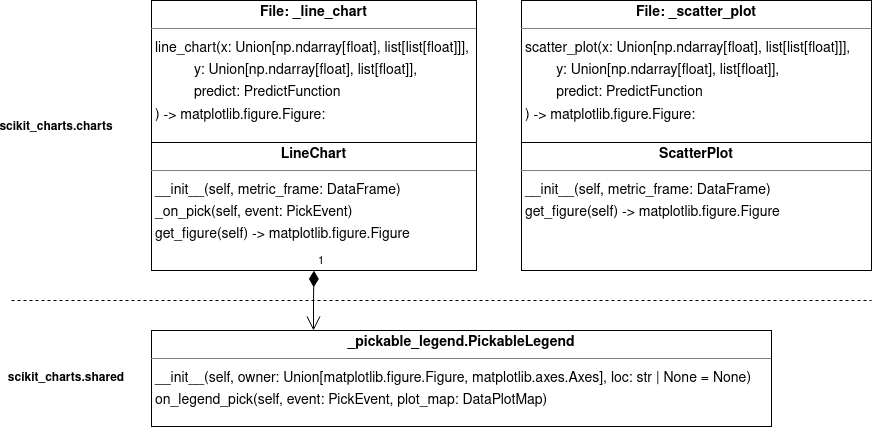
\includegraphics[width=\textwidth]{images/uml_scatter_line_chart.png}
    \caption{Klassendiagramm von Linien- und Streudiagramm}
    \label{fig:uml_line_scatter}
\end{figure}

\subsection{Erstellung des Streudiagramms}
\label{subsec:impl_scatter}
%   - Keine Implementierung von Zoom / Bewegen des Diagramms -> Wird bereits automatisch in interaktiven Umgebungen von Matlab unterstützt
% - wie konfiguriert man interaktivität in Matplotlib
\noindent Die Implementierung des Streudiagramms konnte rein durch die von Matplot zur Verfügung gestellten Funktionen erfolgen. Das grundlegende Diagramm kann mittels eines einzelnen Funktionsaufruf erstellt werden. Sowohl die 45°-Linie als auch das Gitter im Hintergrund können direkt über das Axes-Objekt konfiguriert werden. Der Zoom, sowie die Bewegung des angezeigten Bereiches im Diagramm werden von Matplot out-of-the-box zur Verfügung gestellt. Dafür muss das Diagramm mit einem interaktiven Backend von Matplot gestartet werden.

\subsection{Backends in Matplot}
\label{subsec:impl_backend}
%   - Weitere Abhängigkeit ipympl um dynamische Interaktion in Jupyter zu unterstützen -> Aktivieren mittels %matplotlib widget
\noindent Bei den Backends\footnote{https://matplotlib.org/stable/users/explain/backends.html} von Matplot handelt es sich um Implementierungen der Darstellung für verschiedene grafische Ausgaben. Diese sind entweder statisch für Dateien (PNG, SVG, ...) oder interaktiv basierend auf verschiedenen GUI-Plattformen. In den meisten Fällen wählt die Bibliothek automatisch das passende interaktive Backend für die aktuelle Plattform. Die IDE Pycharm, sowie Jupyter Notebook benötigen jedoch weitere Konfigurationen. In Pycharm muss das passende Backend der aktuellen Plattform mithilfe von `matplotlib.use(...)` konfiguriert werden. Ansonsten wird standardmäßig ein nicht interaktives Backend ausgewählt. Um die Interaktivität in Jupyter Notebook zu ermöglichen wurde eine neue Abhängigkeit auf \emph{ipympl} zum Projekt hinzugefügt. Dabei handelt es sich um ein Matplot Backend für Jupyter Notebook. Anwender:innen können dieses Backend in Jupyter Notebook durch das Einfügen der Zeile \emph{\%matplotlib widget} aktivieren. 

\subsection{Liniendiagramm und Hilfsklassen}
\label{subsec:impl_linien_helper}
\noindent Liniendiagramme werden in Matplot explizit unterstützt. Dafür kann die \emph{plot}-Funktion verwendet werden. Für die interaktive Legende wird jedoch eine Hilfsklasse benötigt. Daher wurde eine Klasse \emph{PickableLegend} erstellt. Diese kümmert sich um das dynamische Ausblenden von Linien durch das Klicken auf den jeweiligen Eintrag in der Legende. Unterstützt wird dabei jedes Figure- oder Axes-Objekt, auf welchem bereits Daten dargestellt wurden. Während der Instantiierung der PickableLegend wird für diese Figure/Axes eine neue Legende erstellt. Diese ist konfiguriert um \emph{on\_pick} Events für Matplot zu generieren. In der Liniendiagrammklasse wird auf diese Events\linebreak reagiert. Wenn ein on\_pick-Event erkannt wird, erfolgt ein Aufruf von \emph{legend\_pic} in der PickableLegend. Diese kümmert sich um das ausblenden der Daten basierend auf dem gewählten Element. Die mitgegebene Map gibt dabei an, welche dargestellten Daten zu welchem Legendeneintrag passen.

\subsection{Matplot Interaktivität und der Garbage-Collector}
\label{subsec:impl_interact_problems}
%   - Click-Events -> Schwer zu koppeln da aktivert werden muss -> Schwer richtige Referenzen zu bekommen + Koppeln mit anderen Daten eine herausforderung
%   - Herausforderung von Referenzen -> Müssen gehalten werden damit interaktivität (Widgets) funtkioniert -> Implementierungen müssen deshalb als Klassen erstellt werden
\noindent Eine Herausforderung während der Implementierung stellte der Lebenszyklus von Python-Objekten dar. Referenzen auf Callback, dargestellte Daten sowie Legende müssen während der gesamten Lebensdauer der Darstellung gespeichert werden. Passiert dies nicht, kann es sein, dass die Objekte vom Garbage Collector entfernt werden. In diesem Fall geht die Interaktivität verloren. Aus diesem Grund sind alle dynamischen UI-Elemente als Klassen implementiert.

\pagebreak

\section{Implementierung des Blasendiagramms}
\label{sec:impl_bubble}

Der Fokus beim Blasendiagramm lag auf dessen hoher Konfigurierbarkeit. Aus diesem Grund einstanden während dessen Entwicklung die meisten Hilfsklassen und Funktionen. Dies ist auch in dem UML-Diagramm des Diagramms in Abbildung \ref{fig:uml_bubble} ersichtlich.

\begin{figure}[H]
    \centering
    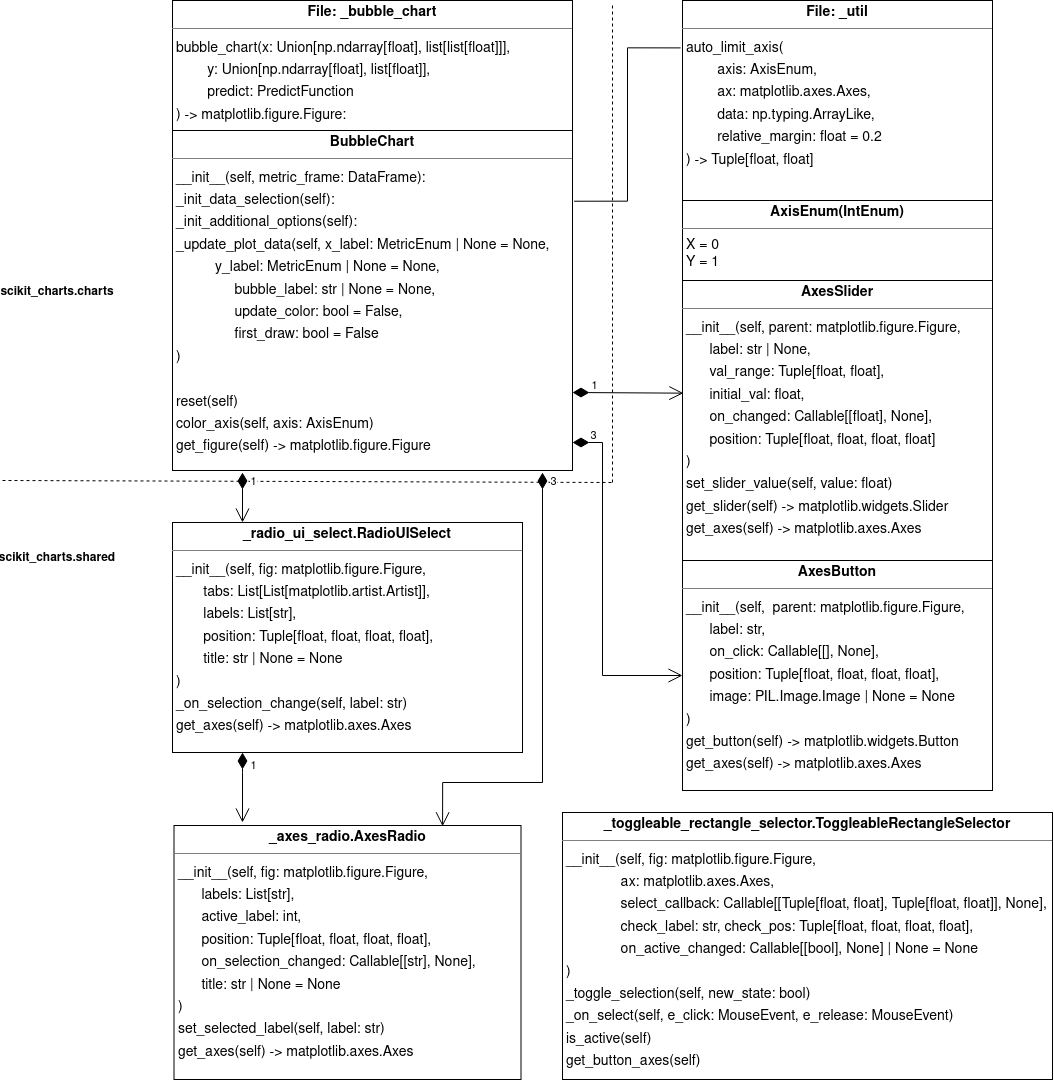
\includegraphics[width=\textwidth]{images/uml_bubble_chart.png}
    \caption{Klassendiagramm des Blasendiagramms}
    \label{fig:uml_bubble}
\end{figure}

\subsection{Hilfsklassen des Blasendiagramms}
\label{subsec:impl_linien_helper}
% - Selektierung von Werten für Achsen
% - Mehrere zusätzliche UI-Elemente (RadioSelect, Axes impls)
Während der Implementierung des Blasendiagramms stellten sich gleich mehrere\linebreak Herausforderungen auf einmal. Die Erste war die Auswahl der Metriken für Achsen und Blasengröße. Da Matplot kein Drop-Down-Menü zur Verfügung stellt, erfolgt die Auswahl über Radio-Buttons. Diese werden in einer Seitenleiste neben dem Diagramm angezeigt. Für die Radio-Buttons wurde eine eigene Hilfsklasse namens \emph{AxesRadio} erstellt. Solche Hilfsklassen, mit dem Namensschema \emph{Axes<UI-Element>} existieren in der Bibliothek für verschiedene UI-Elemente. Beispielsweise auch für Buttons und Slider. Es handelt sich dabei bei allen um einfache Wrapper um die jeweilige Klasse aus Matplot. Diese Hilfsklassen kümmern sich intern um die Positionierung und Konfiguration der Matplot Objekte, sowie das Halten der notwendigen Referenzen. Dadurch wird die Komplexität und Größe der eigentlichen Diagrammklassen verringert. Sie können außerdem von Anwender:innen in eigenen Implementierungen wiederverwendet werden.

\subsection{Aktualisierung der Daten im Diagramm}
\label{subsec:impl_bubble_data_update}
% - Gebündelte Update-Funktion -> Setzen von Daten + Update des Plots
%   - Aufruf von self._plot_data.remove() für effizienteres löschen als figure.clear
\noindent Die Auswahl eines Wertes in der Seitenleiste führt intern zu einem Update der angezeigten Daten. Dafür wird die \emph{\_update\_plot\_data(...)} Funktion aufgerufen. Diese kümmert sich sowohl um das setzen der internen Attribute als auch um das neue Zeichnen der Daten. Als Argumente wird übergeben, ob und welche Daten sich geändert haben. Gleichbleibende Werte werden nicht aktualisiert. Dadurch werden nur die notwendigen Teile im Diagramm neu aufgezeichnet. Durch das Bündeln in einer einzelnen Funktion bleibt der Aufruf zum Neuzeichnen der Daten konsistent. Um das Zeichnen weiter zu optimieren, werden die gezeichneten Daten zwischengespeichert. Sind diese Daten beim nächsten Aufruf verfügbar, werden sie von dem Figure-Objekt entfernt, anstatt die gesamte Figure zurückzusetzen.

\subsection{Layouting des Blasendiagramms}
\label{subsec:impl_bubble_layout}
% - Layouting der UI-Elemente und Bereiche + Warum so implementiert
%   - Herausforderung: Layouting für buttons + keine DropDownMenüs per default -> Plotly wäre einfacher gewesen
\noindent Eine weitere Herausforderung bei der Entwicklung war das Layout des Diagramms. Die hohe Anzahl an Metriken bedeutet, dass viele Einträge gleichzeitig angezeigt werden müssen. Dementsprechend benötigt die Metrikauswahl viel Platz. Wie in HeuristicLab würde ein Drop-Down-Menü dafür Abhilfe schaffen. Als Alternative dazu, wurde neue Radio-Buttons hinzugefügt, mithilfe welcher die angezeigten Einstellungen gewechselt werden können. Dabei kann zwischen X- sowie Y-Achse, Blasengröße und weiteren Optionen\linebreak gewählt werden. Das ganze wurde in einer Hilfsklasse namens \emph{RadioUISelect} implementiert. Dieses Element versteckt automatisch alle UI-Elemente, welche nicht zum aktuell gewählten Eintrag gehören. Dadurch können die vielen Optionen mit relativ geringen Platzverbrauch angeboten werden.

\subsection{Mausinteraktionen und Datenselektierung}
\label{subsec:impl_mouse}

\noindent Das Blasendiagramm in HeuristicLab unterstützt die Selektion und Manipulation einzelner Blasen mithilfe der Maus. Die Implementierung dieser Funktion war ebenfalls für Scikit-charts angedacht. Die Implementierung musste jedoch aus zeitlichen Gründen abgebrochen werden. Das Problem war die Färbung sowie Ausblendung einzelner Datenpunkte. Die bestehende Implementierung führte dabei zu Problem beim Wechseln der angezeigten Metriken. Die Bereichsauswahl selbst, wird explizit von Matplot unterstützt. Dafür werden sogenannte Selektoren bereitgestellt. Diese können zu einem Figure- oder Axes-Objekt hinzugefügt werden. Über einen Callback kann am Ende einer Auswahl auf den gewählten Bereich reagiert werden. Da die Bereichsauswahl nicht dauerhaft aktiv sein soll, ist es notwendig diese umzuschalten. Dafür wurde eine Hilfsklasse namens \emph{ToggleableRectangleSelector} implementiert. Diese fügt zusätzlich zu einem Selektor eine Checkbox in das Diagramm ein. Beim umschalten dieser Checkbox wird ebenfalls die Bereichsauswahl umgeschaltet und der zuletzt gewählte Bereich ausgeblendet. Um auf die Auswahl reagieren zu können, werden zwei Callbacks übergeben. Der eine erhält die minimale und maximale Position des Bereiches, sobald sich dieser ändert. Der Bereich kann dadurch in der Diagrammklasse abgespeichert werden. Der andere Callback reagiert auf das Umschalten des Selectors. Dadurch können gespeicherte Werte in der Klasse wieder invalidiert werden.


\section{Implementierung des Schnittdiagramms}
\label{sec:impl_partial_dependency}

Beim Schnittdiagramm handelte es sich um die wohl komplexeste Diagrammimplementierung. Die Herausforderungen lagen dabei bei der Berechnung und Verwaltung der Daten, sowie der komplexen Interaktivität. Das Diagramm wurde deshalb in zwei\linebreak Klassen unterteilt. Zusätzlich wurde eine weitere Hilfsklasse dafür entwickelt.

\begin{figure}[H]
    \centering
    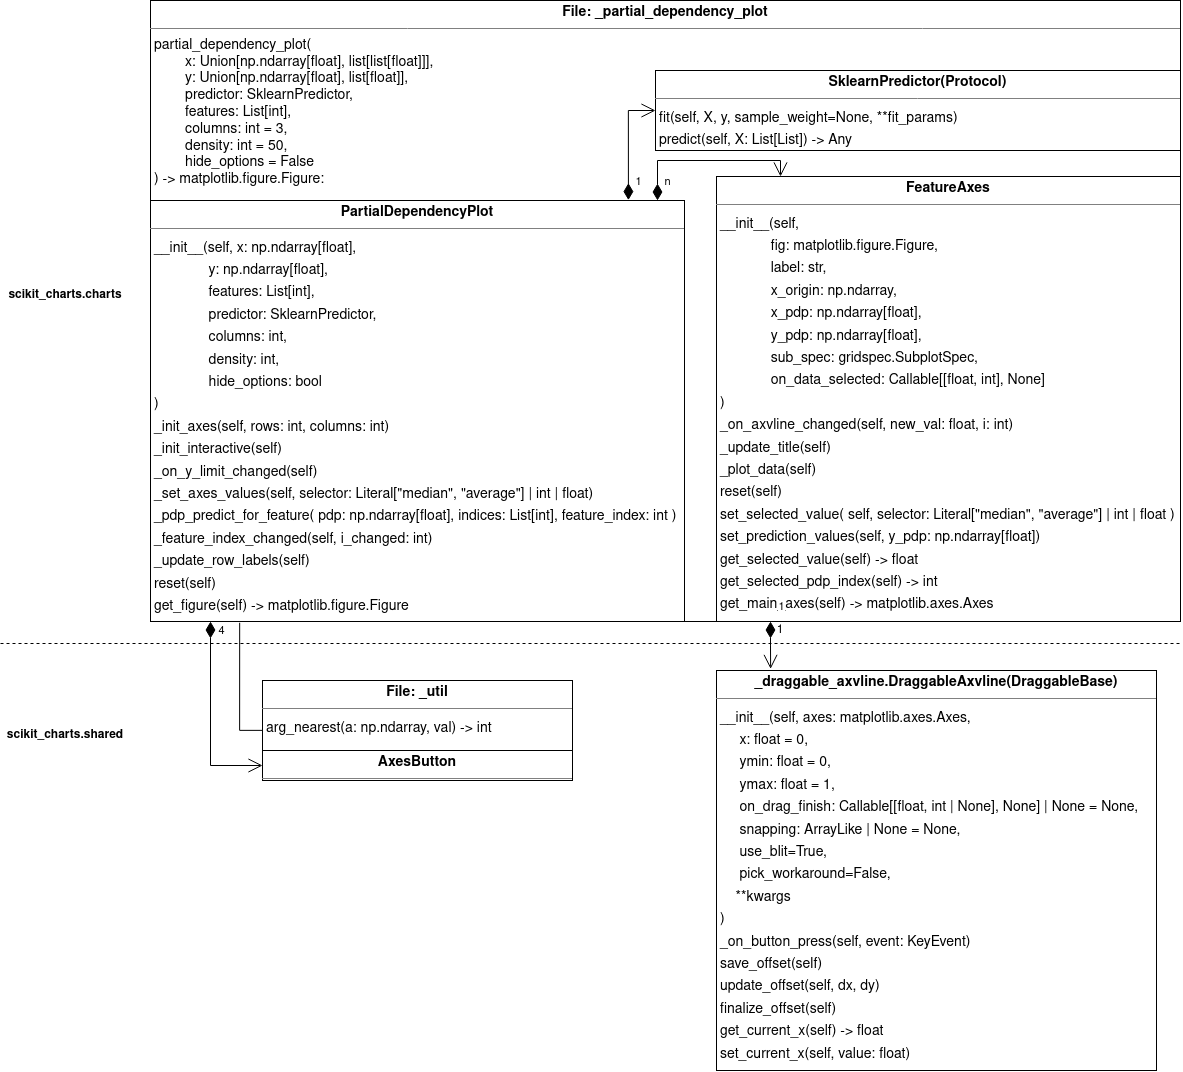
\includegraphics[width=0.95\textwidth]{images/uml_partial_dependence.png}
    \caption{Klassendiagramm des Schnittdiagramms}
    \label{fig:uml_partial_dependence}
\end{figure}

\subsection{Berechnung der Abhängigkeiten}
\label{subsec:pdp_calculation_visualization}
% - SklearnPredictor
Zur Berechnung der \emph{partial dependence} (Abschnitt \ref{sec:partial_dependence}) wird die Funktion\linebreak \emph{sklearn.inspection.partial\_dependence(..)} verwendet. Dafür wird ein in Scikit-learn trainiertes Modell benötigt. Da Scikit-learn dafür keine Typinformationen bereitstellt, wird eine eigene \emph{Protocol}-Klasse implementiert. Ein \emph{Protocol}\footnote{https://peps.python.org/pep-0544/} in Python beschreibt den Typ eines Objektes basierend auf dessen Struktur. Das Schnittdiagramm benötigt daher einen \emph{SklearnPredictor}. Diese Protocolklasse definiert ein Objekt welches eine \emph{fit} und \emph{predict} Funktion besitzt. Diese werden mindestens für die partial\_dependence-Funktion benötigt.\\\\
% - Scikitlearn für Berechnung von Partial-Dependence
% Index von Feature-Wert zum Zugriff auf Predict-Liste
% Reihenfolge für Zugriff die gleiche wie originale Indicies
% Feature-Werte + Werte aus Predict-Liste werden in Kacheln angezeigt
\noindent Das Ergebnis der partial\_dependence-Funktion ist eine Map ähnliche Datenstruktur für eine angegebene Liste an Einflussvariablen. Ein Eintrag im Ergebnis beinhaltet mögliche Werte für alle gewählten Einflussvariablen. Ein weiterer Eintrag ist eine $m^n$ tief geschachtelte Liste, welche die Vorhersagen für die Wert-Kombinationen\linebreak beinhaltet. Variable $n$ beschreibt dabei die Anzahl der gewählten Einflussvariablen. Variable $m$ beschreibt die Anzahl an generierten Werten pro Einflussvariable. Der Zugriff auf das Vorhersagen-Array ($pd$) erfolgt über die Indices der gewählten Variablenwerte: $pd[n_0][n_{...}][n_n]$. Um dementsprechend in einer Wertkombination alle Vorhersagen für\linebreak eine Variable zu erhalten, müssen an der Position dieser Variable alle möglichen Indices gewählt werden. Da dieser Zugriff durch die Komplexität Fehleranfällig ist, wurde er in die Funktion \emph{\_pdp\_predict\_for\_feature(..)} ausgelagert. Diese gibt die Vorhersage für eine Einflussvariable basierend auf den Wert-Indices zurück. Ein Beispiel für den Zugriff in Python ist in der nachfolgenden Tabelle ersichtlich.\\

\begin{table}[H]
\centering
    \begin{tabular}{lll}
        \textbf{Einflussvariable} & \textbf{x1} & \textbf{x2} \\ [0.4cm]
        \textbf{Generierte Werte} & {[}1; 2.5; 3{]} & {[}0; 3; 4{]} \\ [0.4cm]
        \textbf{Generierte Vorhersage (pd)} & \multicolumn{2}{l}{{[}{[}1; 4; 5{]}, {[}2,5; 5,5; 6,5{]}, {[}3; 6; 7{]}{]}} \\ [0.4cm]
        \textbf{Gewählte Variablenwerte} & 2,5 & 4 \\ [0.4cm]
        \textbf{\begin{tabular}[c]{@{}l@{}}Vorhersage basierend auf\\ Wert anderer Variable\end{tabular}} & \begin{tabular}[c]{@{}l@{}}pd{[}:, 2{]} -\textgreater\\ {[}5; 6,5; 7{]}\end{tabular} & \begin{tabular}[c]{@{}l@{}}pd{[}1, :{]} -\textgreater\\ {[}2,5; 5,5; 6,5{]}\end{tabular}
    \end{tabular}
\caption{Beispiel zur Verwendung der Ergebnisse von `partial\_dependence()`}
\label{tab:partial_dependence_result}
\end{table}

% - FeatureAxes für Unterteilung
\noindent Die generierten Werte der Einflussvariablen, sowie die dazugehörigen Vorhersagen, werden in den einzelnen Feldern des Schnittdiagramms angezeigt. Diese sind in der Klasse \emph{FeatureAxes} implementiert. Die Klasse kümmert sich um die gesamte Darstellung für einzelne Einflussvariablen. Zusätzlich zu den generierten Werten, werden auch die Werte der Einflussvariable im Datensatz verwendet. Diese Werte werden als Histogramm über den einzelnen Feldern angezeigt. Zusätzlich wird der originale Datenbereich in den Feldern eingezeichnet.

\subsection{Interaktivität zur Analyse der Abhängigkeiten}
\label{subsec:pdp_interactivity}
% - Interaktivität
%   - Dragable axvline
%   - Auswahl der neuen Vorhersagen basierend auf neuer Auswahl -> Setzen in Achsen + Setzen in Label der Reihen
%   - Snapping
\noindent Die Hauptfunktion des Schnittdiagramms ist die interaktive Darstellung der Abhängigkeiten von Einflussvariablen. Dafür müssen Anwender:innen die Möglichkeit haben, konkrete Werte pro Einflussvariable zu wählen. Dafür wurde die Klasse\linebreak \emph{DraggableAxvline} implementiert. Axvline beschreibt eine Funktion der Matplot Axes-Objekte. Mithilfe dieser wird eine vertikale Linie im Diagramm eingezeichnet. Um das Ziehen dieser Linien zu ermöglichen, wird die Matplot Klasse \emph{DraggableBase}\footnote{https://matplotlib.org/stable/api/offsetbox\_api.html\#matplotlib.offsetbox.DraggableBase} erweitert. Diese kümmert sich um das Registrieren der notwendigen Eventhandler. Des Weiteren definiert DraggableBase Funktionen, über welche auf die Mausbewegungen reagiert werden kann. DraggableAxvline bietet zusätzlich die Möglichkeit, die gewählten Werte auf eine Liste von bestimmten Werten zu begrenzen. Dafür wird am Ende des Ziehens der Linie der näheste Werte in der Liste gewählt. Das ist notwendig, da nur von partial\_dependence generierte Werte zur Auswahl stehen dürfen. Der Index dieses Wertes ist weiterführend notwendig, für die Auswahl der korrekten generierten Vorhersage.\\\\
\noindent Das Schnittdiagramm reagiert auf die Änderungen eines gewählten Wertes über einen Callback. Dieser erhält den Index der Einflussvariable, sowie den Index des gewählten Wertes. Mithilfe dieser werden die möglichen Vorhersagen aller anderen Felder\linebreak aktualisiert. Danach wird der Wert der Vorhersage am Beginn der Zeilen aktualisiert.

\subsection{Einschränkungen des Matplot Eventsystems}
\label{sec:pdp_matplot_einschraenkung}
\noindent Während der Implementierung der DraggableAxvline wurde eine Einschränkung des Matplot Eventsystems sichtbar. Das Pick-Event eines Axes-Objekt wird nicht korrekt weitergeleitet, wenn mehrere Axes-Instanzen in einer Figure existieren. Das führt dazu, dass das Verschieben der Linie nicht funktioniert. DraggableBase verwendet das Pick-Event intern um den Start der Bewegung zu erkennen. Deswegen wurde ein Workaround in die DraggableAxvline implementiert. Dabei wird für das Figure-Objekt ein Button-Press-Event registriert. Wird ein Knopf gedrückt, erfolgt die Prüfung ob es sich dabei um einen Mausklick auf die Linie handelt. Ist das der Fall, wird \emph{pick} für die Linie aufgerufen. Dadurch wird das Verschieben der Linie vom Code aus gestartet.

\subsection{Konfiguration und Performance}
\label{subsec:pdp_config_performance}
% - Verbesserungen der Performance -> Direkt ndarray statt DataFrame -> keine Metric berecchnung da DPD alles beinhaltet
% - Beschreibung zusätlicher Argumente und Interaktion
\noindent Die Funktion des Schnittdiagramms weicht von den anderen Diagrammimplementierungen ab. Das liegt an Einschränkungen der Implementierung. Zum einen wird ein SklearnPredictor anstatt einer predict-Funktion benötigt. Zum anderen muss zu Beginn eine Liste an Indices übergeben werden. Diese Entsprechen den Indices der Einflussvariablen aus dem Argument \emph{x}, welche im Diagramm enthalten sein sollen. Es ist in den meisten Fällen nicht möglich, alle Einflussvariablen gleichzeitig anzuzeigen. Das liegt an der Menge an generierten Daten von partial\_dependence. Je mehr Einflussvariablen angegeben werden, desto größer wird die generierte Datenstruktur. Im Extremfall kann die Berechnung fehlschlagen, da Numpy mehre Gigabyte an Speicher für das Array\linebreak allokieren möchte.\\\\
\noindent Eine weitere Möglichkeit die Anzahl an generierten Werte zu Beeinflussen bietet das \emph{density} Argument. Dieses beschreibt wie viele Werte pro Einflussvariable generiert\linebreak werden. Mehr Werte bedeuten dabei eine längere Berechnungsdauer und höheren Speicheraufwand. Dafür werden auch die dargestellten Abhängigkeiten genauer. Scikit-learn verwendet als Standardwert für die Berechnung 100. In der Bibliothek wird standardmäßig 50 verwendet, um mehr Einflussvariablen gleichzeitig anzeigen zu können.\\\\
\noindent Zusätzlich zu diesen beiden Argumenten bietet das Schnittdiagramm noch zwei weitere Argumente, um das Layout zu konfigurieren. Durch das \emph{columns} Argument kann die\linebreak Anzahl der Spalten für die einzelnen Felder eingestellt werden. Mithilfe von \emph{hide\_options} können die\linebreak dynamischen Konfigurationen des Diagramms ausgeblendet werden. Die dynamischen Interaktionen sind dabei von HeuristicLab inspiriert. Über eine Seitenleiste kann für alle Einflussvariablen der Median oder Durchschnitt basierend auf den Werten im Datensatz ausgewählt werden. Außerdem gibt es die Möglichkeit, den Wertebereich für die Y-Achse zu konfigurieren. Zuletzt wird noch einen Knopf angeboten, welcher das Diagramm auf die initialen Werte zurücksetzt.

\section{Testen der Implementierung}
\label{sec:impl_tests}

Um die Funktionalität zu validieren wurden Unittests implementiert. Diese Umfassen alle Funktionen des \emph{shared}- sowie des \emph{metrics}-Moduls. Im metrics-Modul wird die richtige Berechnung des Metrik-Dataframes sowie die Validierung der Argumente überprüft. Bei der Validierung der Argumente wird ebenfalls geprüft, ob die erwarteten Fehler geworfen werden.\\\\
\noindent Die Diagramme wurden durch manuelle Tests überprüft. Als Umgebung wurde dafür sowohl Jupyter Notebook als auch IPython auf einem Linux-System verwendet. Für die Tests wurde ein Teil des Friedman1 Datensatzes (\parencite{friedman_data}) verwendet. Der verwendete Datensatz enthielt 100 Zeilen mit je 10 Einflussvariablen und einem Zielwert. Zur Vorhersage der Werte wurde sowohl ein statisches Modell als auch ein lineares Regressionsmodell verwendet. Das lineare Regressionsmodell wurde wegen der schnellen Trainingsdauer und Berechnung der Werte gewählt. Das statische Modell sowie die Daten wurden vom Betreuer dieser Arbeit zur Verfügung gestellt. Das statische Modell wird mit der folgenden Funktion beschrieben:

\begin{PythonCode}
def predict_friedman(x: [float]) -> float:
    return 10.01534687044389 * math.sin(3.137809802901138 * x[0] * x[1]) \
        - 0.165196466779569 * x[2] * math.sin(11.89520954531139 * x[0] - 4.424478615506525 * x[3]) \
        + 4.718864748760709 * math.cbrt(math.cos(6.283437605197133 * x[2]) - 1.023099551839108) \
        + 10.03958259409875 * x[3] + 5.104038843356345 * x[4] + 5.948126001166421
\end{PythonCode}

\noindent Eine Eigenschaft dieses Datensatzes ist, dass nur die ersten fünf Einflussvariablen einen signifikanten Einfluss auf den Zielwert haben. Dadurch eignet es sich gut zum Testen des Schnittdiagramms. Bei einem korrekt trainierten Modell, sollte der Einfluss der Variablen 6 bis 10 im Schnittdiagramm annähernd horizontal dargestellt werden.
\chapter{Evaluierung}
\label{cha:evaluation}

Dieses Kapitel präsentiert die Ergebnisse der Arbeit. Dabei werden die finalen\linebreak Diagramme und ihre einzelnen Funktionen präsentiert. Innerhalb der Diagramme wird der in den Testfällen beschriebene Datensatz (Abschnitt \ref{sec:impl_tests}) mit einem daraus erstellten linearen Regressionsmodell dargestellt. Nach der Präsentation der Ergebnisse wird überprüft, ob die implementierten Diagramme die Problemstellung erfolgreich lösen. Im Zuge dessen werden auch mögliche Verbesserungen der Bibliothek hervorgehoben. Alle Ergebnisse werden danach zum Ende des Kapitels als Tabelle zusammengefasst.

\section{Präsentation der Ergebnisse}
\label{sec:eval_presentation}

Die wichtigsten Ergebnisse der Arbeit sind die Implementierungen der Diagramme.\linebreak Der Sourcecode der Bibliothek selbst ist auf GitHub unter der Adresse\linebreak \emph{https://github.com/Pystronic/scikit-charts} verfügbar.

\begin{figure}[H]
    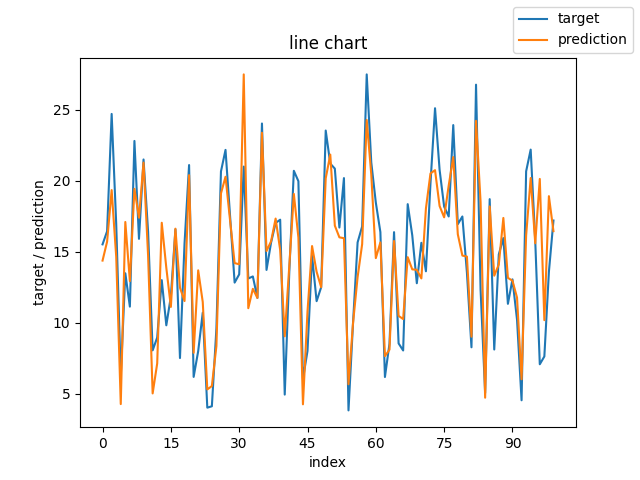
\includegraphics[width=0.5\textwidth]{images/exm_liniendiagramm.png}
    \hfill
    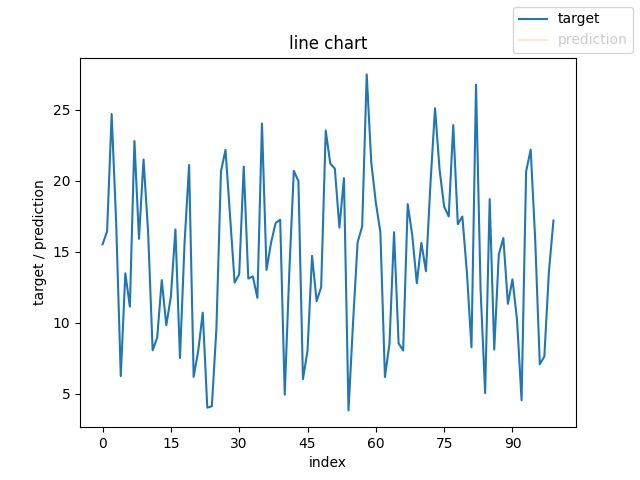
\includegraphics[width=0.5\textwidth]{images/exm_liniendiagramm_interacted.png}
    \caption{Ergebnis des Liniendiagramms und dessen Interaktion}
    \label{fig:eval_line_chart}
\end{figure}

\noindent Das Liniendiagramm konnte mit mit demselben Funktionen wie in HeuristicLab umgesetzt werden. Einzig die Unterscheidung zwischen Test- und Trainingsdaten wird nicht unterstützt. Es kann ohne weitere Konfiguration angwendet werden, um Muster\linebreak basierend auf dem Index in den Zielwerten zu finden. Dieses Muster kann dann mit dem Ergebnissen der Vorhersage verglichen werden. Dabei erweitert das Diagramm die\linebreak Standardimplementierung des Liniendiagramms um das dynamische Ausblenden von Daten über die Legende. Diese Funktion ist in Abbildung \ref{fig:eval_line_chart} ersichtlich. In dieser werden die Vorhersagen zwischen den beiden Darstellungen ausgeblendet.

\begin{figure}[H]
    \centering
    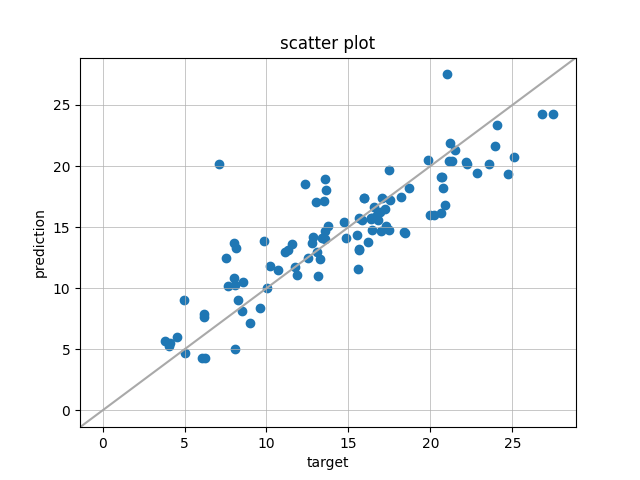
\includegraphics[width=0.5\textwidth]{images/exm_scatterplot.png}
    \caption{Ergebnis des Streudiagramms}
    \label{fig:eval_scatter_plott}
\end{figure}

\noindent Das finale Streudiagramm stellt eine konfigurierte Variante der Standardimplementierung aus Matplot dar. Dabei besitzt das Diagramm standardmäßig ein Gitter, sowie die 45° Linie in der Darstellung. Es ermöglicht Anwender:innen einen schnellen und präzisen Vergleich der Vorhersagen gegenüber den Zielwerten.

\begin{figure}[H]
    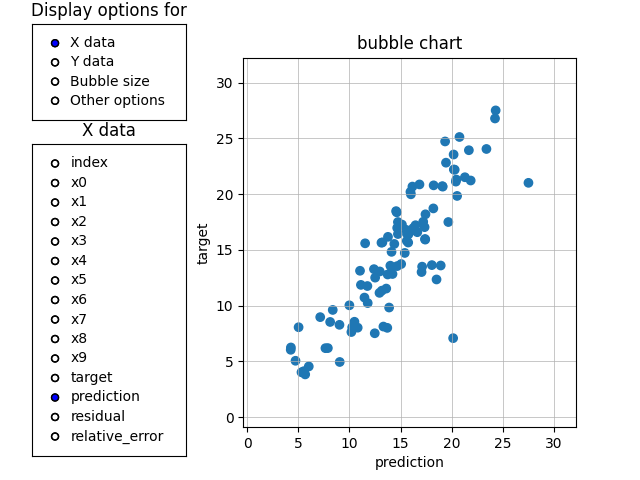
\includegraphics[width=0.5\textwidth]{images/exm_bubblechart.png}
    \hfill
    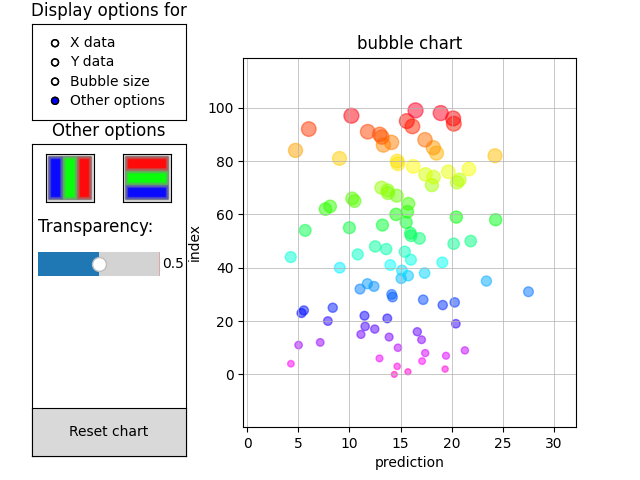
\includegraphics[width=0.5\textwidth]{images/exm_bubblechart_interacted.png}
    \caption{Ergebnis des Blasendiagramms und dessen Interaktionen}
    \label{fig:eval_bubble_chart}
\end{figure}

\noindent Mit der finalen Implementierung des Blasendiagramms wird eine Erweiterung des\linebreak standardmäßigen Streudiagramms zur Verfügung gestellt. Über die Blasengröße ermöglicht das Diagramm den Vergleich dreier Metriken auf einmal. Im Zentrum steht dabei die dynamische Auswahl der Metrik für die einzelnen Achsen und die Blasengröße. Durch diese wird ein interaktiver Vergleich ermöglicht, ohne jedes Mal ein neues Diagramm zu generieren. Die Färbung erlaubt es, die Blasen über die Werte einer Metrik weiter hervorzuheben. Da diese Färbung beim Wechseln der Achsen-Metrik erhalten bleibt, ermöglicht sie es ebenfalls eine vierte Dimension für Vergleiche einzubauen. Mithilfe des Sliders für die Transparenz ist es möglich die Dichte der Datenpunkte zu überprüfen. Dabei werden bei einer hohen Transparenz dichte Punkte durch die Überlappung stärker angezeigt. Zuletzt gibt es noch die Möglichkeit das gesamte Diagramm auf die initialen Werte zurückzusetzen. Das betrifft sowohl für die gesetzten Metriken, als auch die Färbung und Transparenz.

\begin{figure}[H]
    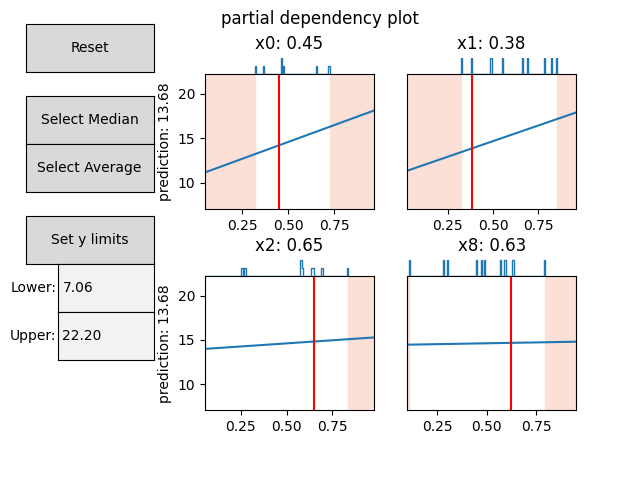
\includegraphics[width=0.5\textwidth]{images/exm_schnittdiagramm.png}
    \hfill
    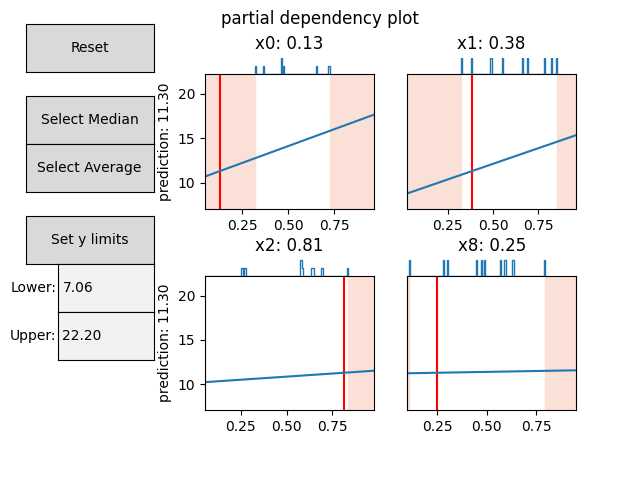
\includegraphics[width=0.5\textwidth]{images/exm_schnittdiagramm_after_moving.png}
    \caption{Ergebnis des Schnittdiagramms und dessen Interaktionen}
    \label{fig:eval_partial_dependency}
\end{figure}

\noindent Das finale Schnittdiagramms ermöglicht es, den Einfluss mehrerer Einflussvariablen\linebreak dynamisch zu analysieren. Dabei werden beim Aufruf des Diagramms die Traningsdaten des in Scikit-learn trainierten Modelles, sowie die Indices der darzustellenden Einflussvariablen übergeben. Der Einfluss der einzelnen Variablen wird daraufhin berechnet und in Feldern dargestellt. Die blaue Linie in der Mitte der Felder zeigt dabei das Verhältnis des Einflusses an. Das Verhältnis ist dabei die Relation zwischen den möglichen Werten auf der X-Achse und den Vorhersagen auf der Y-Achse. Über den einzelnen Feldern ist die Dichte der Werte im originalen Datensatz eingezeichnet. Diese wird als Histogramm dargestellt. Bereiche welche sich nicht im originalen Datensatz befinden, werden in den Felder mit einer roten Färbung hinterlegt. Die rote vertikale Linie der Felder zeigt den aktuell gewählten Wert für eine Variable an.\\\\
\noindent Sowohl die berechnete Vorhersage am Beginn der Reihen, als auch das dargestellte Verhältnis ist abhängig von den aktuell gewählten Werten. Vorhersage und\linebreak dargestellter Einfluss werden beim Verändern der Auswahl automatisch aktualisiert. Die Auswahl eines Wertes erfolgt durch das Verschieben der Linie mithilfe der Maus. Alternativ kann der gewählte Werte für alle Einflussvariablen über die Knöpfe in der Seitenleiste gesetzt werden. In Abbildung \ref{fig:eval_partial_dependency} ist der Unterschied vor und nach dem Verschieben ersichtlich. In der Seitenleiste ist es ebenfalls möglich, den Wertebereich für die\linebreak Y-Achse anzupassen. Die Anzahl der dargestellten Spalten, sowie die Anzahl an generierten Werte, pro Variable können nur beim Aufruf der Funktion konfiguriert werden. Es ist außerdem möglich, die Seitenleiste beim Aufruf des Diagramms zu deaktivieren.

\pagebreak

\subsection{Ergebnisse außerhalb der Aufgabenstellung}
\label{subsec:eval_other_results}

\noindent Neben den Diagrammen wurde auch noch weitere Ergebnisse erzielt. Die Implementierung der Metriken kann auch außerhalb der Bibliothek angewandt werden. Dasselbe gilt für die geteilten Hilfsklassen der einzelnen Diagramme. Diese können bei der Erstellung eigener interaktiver Visualisierungen von Anwender:innen genutzt werden. Bei diesen Hilfsklassen handelt es sich um Wrapper für Matplot UI-Elemente. Diese\linebreak vereinfachen die Platzierung und Erstellung der Elemente in einem Diagramm. Außerdem werden auch erweiterte interaktive Elemente, welche nicht standardmäßig existieren, zur Verfügung stehen.

\section{Gegenüberstellung der Ergebnisse mit der Problemstellung}
\label{sec:eval_problemstellung}

In der Problemstellung (Abschnitt \ref{sec:Problemstellung}) werden Anforderungen an Bibliotheken zur\linebreak Visualisierung von Regressionsmodellen definiert. Dabei können drei konkrete\linebreak Anforderungen zusammengefasst werden:
\begin{enumerate}
    \item Keine Notwendigkeit von spezifisches Wissen.
    \item Einfache Integration der Diagramme.
    \item Dynamische Analysen durch Interaktivität.
\end{enumerate}

\vspace{\baselineskip}

\noindent Punkt 1 wird mit Einschränkungen erfüllt. Scikit-chart abstrahiert Matplot über den Aufruf des Diagramms. Es kann jedoch notwendig sein einige Einstellungen zu treffen, um Interaktivität der Diagramme zu aktivieren. Diese benötigen Matplot spezifisches wissen. Das ist vor Allem in Jupyter Notebook der Fall. Die notwendigen Schritte sind jedoch in Abschnitt \ref{subsec:impl_backend} beschrieben.\\\\
\noindent Punkt 2 wird von der Bibliothek erfüllt. Durch die Implementierung über Matplot können die Diagramme auf unterschiedlichen Plattformen integriert werden. Drei der Vier Diagramme können Regressionsmodelle unabhängig der verwendeten Bibliothek\linebreak darstellen. Einzig das Schnittdiagramm besitzt die Einschränkung auf ein mit Scikit-learn trainiertes Modell. Der Aufruf der Diagramme selbst, ist von den Funktionen in Scikit-learn inspiriert. Durch die ähnliche Reihenfolge der Argumente können sich Anwender:innen von Scikit-learn leichter in die Bibliothek einfinden. Zuletzt unterstützt die konsequente Verwendung von eingebetteter Dokumentation sowie von Typinformationen die Anwender:innen bei der Integration.\\\\
\noindent Punkt 3 wird über Blasendiagramm und Schnittdiagramm unterstützt. Beide Diagramme ermöglichen eine interaktive Analyse eines Regressionsmodells sowie des dazugehörigen Datensatz. Die Interaktivität vereinfacht es dabei mögliche Zusammenhänge zwischen den Daten zu erkennen. Liniendiagramm und Streudiagramm erfüllen diesen Punkt jedoch nicht, wegen ihrer geringen Interaktivität.

\section{Gegenüberstellung der Ergebnisse mit der Zielsetzung}
\label{sec:eval_zielvorgabe}

Die Zielsetzung (Abschnitt \ref{sec:Zielsetzung}) wurden umgesetzt. Die Funktionalitäten aus HeuristicLab wurden jedoch nicht komplett übernommen. Die Bibliothek unterstützt\linebreak das Sammeln der Metriken, welche in aus HeuristicLab identifiziert wurden. Die Implementierungen der Diagramme orientieren sich an HeuristicLab, besitzen jedoch einige Einschränkungen. Konkret fehlen Funktionalitäten bei Blasendiagramm und Schnittdiagramm. Beim Blasendiagramm sind es die Auswahl von Datenpunkten, sowie das Färben und Verstecken der gewählten Punkte. Des Weiteren gibt wurde der Jitter sowie die weitere Anpassung der gewählten Blasengröße nicht implementiert. Beim Schnittdiagramm fehlt die dynamische Auswahl der Einflussvariablen sowie die dynamische Änderung der Spaltenanzahl. Es fehlt ebenfalls das Setzen der Variablenwerte auf eine gewisse Zeile im Datensatz. Bei den restlichen Punkten der Zielsetzung gab es keine Einschränkungen. Mithilfe von Poetry, kann aus dem Projekt ein Python-Paket gebaut werden. Dadurch kann die Bibliothek entweder systemweit installiert oder für bestimmte Projekt hinzugefügt werden. Die Unterstützung von Scikit-learn wurde sogar überfüllt, da Liniendiagramm, Streudiagramm und Blasendiagramm beliebige Modelle unter-stützen. Die Integration in Jupyter Notebooks wurde ebenfalls getestet und notwendige Konfigurationen in Abschnitt \ref{subsec:impl_backend} beschrieben.

\section{Mögliche Verbesserungen der Bibliothek}
\label{sec:eval_improvements}

Die bestehende Implementierung unterstützt alle notwendigen Anforderungen.\linebreak Trotzdem könnten noch verschiedene Verbesserungen getroffen werden, um den Wert der Bibliothek für Anwender:innen zu erhöhen. Diese Verbesserungen umfassen Usability, Performance, Stabilität und Flexibilität.\\\\
\noindent Die möglichen Verbesserungen in der Usability auf die Interaktion mit den einzelnen Diagrammen. Bei der interaktiven Legende, den RadioButtons und roten Linie im Schnittdiagramm sollte der Cursor auf eine Hand geändert werden. Dadurch wird die Interaktivität dieser Elemente impliziert. Weiters könnte das Layout der Diagramme verbessert werden. Dabei sollte die Seitenleiste verkleinert werden, was eine eigene Drop-Down-Implementierung erforderlich macht. Zuletzt könnte noch die Skalierung in den Diagrammen verbessert werden. Aktuell skalieren Textgrößen und die Größe der UI-Elemente nicht korrekt mit der Fenstergröße.\\\\
\noindent Für eine bessere Performance können drei Punkte in Betracht gezogen werden. Zuerst könnte eine Alternative zu Pandas-Dataframes für die Speicherungen der Metriken verwendet werden. Das liegt daran, dass der Zugriff auf einen Dataframe ist langsamer ist als die Verwendung von Numpy-Arrays. Weiters könnte auf die Verwendung eines Dataframes im Liniendiagramm und Schnittdiagramm verzichtet werden. Diese benötigen zur Darstellung nur einen Teil der Metriken. Eine weitere mögliche Verbesserung könnte auch die Implementierung von \emph{blitting}\footnote{https://matplotlib.org/stable/tutorials/advanced/blitting.html} darstellen. Dabei werden alle statischen Elemente einmalig gezeichnet und als Bild abgespeichert. Bei jeder Aktualisierung\linebreak werden nur noch das gespeicherte Bild und die aktualisierten Elemente gezeichnet. Die letzte mögliche Verbesserung ist bei der Berechnung der partial dependence möglich. Diese stellt aktuell die größte Einschränkung im Schnittdiagramm dar. Eine schnellere Berechnung würde die Anzahl der darstellbaren Einflussvariablen erhöhen. Dafür könnte entweder die Implementierung in Scikit-learn auf Verbesserungen geprüft werden oder eine eigene Implementierung erstellt werden. Die eigene Implementierung hätte den Vorteil, dass sie genau den Anforderungen von Scikit-charts entsprechen würde. Dafür würde diese ebenfalls den Wartungsaufwand der Bibliothek erhöhen.\\\\
\noindent Die Verbesserungen der Stabilität umfassen vor Allem eine höhere Anzahl an automatisierten Tests. Diese könnten mögliche Fehler bei den Diagrammen genauer vorbeugen. Außerdem sollten für zur Validierung der Darstellung Visual-Regression Tests\linebreak \parencite{VisualRegression} in Erwägung gezogen werden. Dabei ein Bild eines korrekt dargestellten Diagramms mit neueren Bildern der Diagramme verglichen. Die Testfälle stellen dadurch die konsistente Darstellung der Daten sicher. Als ein weiterer Punkt sollte noch geprüft werden, ob die fehlende Rückgabe des Diagramm-Objektes zu Problemen während der Ausführung führen kann. In den aktuellen, kurzen Tests konnte das noch nicht eindeutig festgestellt werden. Zuletzt könnten noch genauere Validierungen für die Argumente von Funktionen durchgeführt werden. Dies würde vor allem beim Hinzufügen neuer Parameter notwendig und ermöglicht es Laufzeitfehler besser vorbeugen.\\\\
\noindent Als letzter Punkt könnte noch die Flexibilität der Bibliothek verbessert werden. Dafür würden mehr Parameter in den Hilfsklassen hinzugefügt werden. Diese sollten die Konfiguration der optionalen Parameter von Matplot ermöglichen. Dadurch wird die Verwendung für eigene Diagrammimplementierungen durch Anwender:innen verbessert werden. Liniendiagramm und Streudiagramm könnten außerdem allgemein definiert werden, um beliebige Daten der Anwender:innen damit darzustellen. Zuletzt könnte das Blasendiagramm erweitert werden, sodass Anwender:innen eigene Metriken definieren und\linebreak vergleichen können. Dadurch würde sichergestellt werden, dass durch die beschränkten Metriken keine Einschränkungen für Anwender:innen entstehen.

\section{Reflexion}
\label{sec:ausblick}

Aus persönlicher Sicht ist das Ergebnis der Bachelorarbeit zufriedenstellend. Die Durchführung der Arbeit hätte jedoch besser laufen können. Trotz einiger privater Herausforderungen wurde die verfügbare Zeit eher suboptimal genutzt. Die Arbeit könnte dementsprechend noch weiter ausgebaut werden. Inhaltlich kann die Arbeit jedoch trotzdem als Einstieg in verschiedene Themen genutzt werden. Sie bietet Leser:innen grundlegendes Wissen über Regressionmodelle und Datenanalyse. Das Hauptthema stellt\linebreak jedoch eindeutig die Visualisierung dar. Im Bezug darauf kann die Bibliothek als ein Einstieg in die Verwendung von Matplot verwendet werden. Dabei unterstützen die aufgelisteten Probleme, welche bei der Nutzung der Bibliothek entstehen können. Im Bezug\linebreak auf die Implementierung wurde zwar die grundlegende Zielsetzung erfüllt,\linebreak dennoch existiert unausgeschöpften Potenzial. Somit liegt es an der Zeit nach der Arbeit, dieses Potenzial weiter auszuschöpfen. 

% Notes:
% - Probleme / Herausforderungen beim Entwickeln:
%   - Jupyter notebook -> Diagramme werden zweimal angezeigt -> Jupyter zeigt generierte matplot-figures automatisch an -> Lösung: Strichpunkt am einde von Funktionsaufruf oder rückgabewert abspeichern -> Kein .show aufruf notwendig

% Aufgaben:
% - Feinschliff
%   - Konsequentes Großschreiben von Bibliotheksnamen
%   - Fehler ausbessern + Schreibweise prüfen
%   - References zu Biliotheken als Bib-Reference zu Software
%   - Literaturverzeichnis fixen
%   - Prüfen wegen Emph, ob überall gesetzt

%%%-----------------------------------------------------------------------------
\appendix                                                             % Appendix 
%%%-----------------------------------------------------------------------------

% TODO
%\chapter{Technical Details}
\label{app:TechnicalDetails}



 % Technical supplements
%\chapter{Supplementary Materials}
\label{app:materials}


List of supplementary data submitted to the degree-granting institution for archival storage
(in ZIP format).

% Use this as an example only, adapt the structure to your requirements!

\section{PDF Files}
\begin{FileList}{/}
\fitem{thesis.pdf} Master/Bachelor thesis (complete document)
\end{FileList}

\section{Media Files}
\begin{FileList}{/media}
\fitem{*.ai, *.pdf} Adobe Illustrator files
\fitem{*.jpg, *.png} raster images
\fitem{*.mp3} audio files
\fitem{*.mp4} video files
\end{FileList}


\section{Online Sources (PDF Captures)}
\begin{FileList}{/online-sources}
\fitem{Reliquienschrein-Wikipedia.pdf} \citenobr{WikiReliquienschrein2020}
\end{FileList}




 % Contents of the CD-ROM/DVD
%\chapter{Questionnaire}
\label{app:Questionnaire}





 % Chronological list of changes
%\chapter{\latex Source Code}
\label{app:SourceCode}

 % Source text of this document

%%%-----------------------------------------------------------------------------
\backmatter                           % Back part (bibliography, glossary, etc.)
%%%-----------------------------------------------------------------------------

\MakeBibliography % References
%%% Uncomment if actually used
%\makeglossaries

% ToDo:

\printglossary

%\chapter{Abkürzungsverzeichnis}
%\begin{acronym}[FER]
%\end{acronym}

% Eingabe       Ausgabe
% \acro{ecu}[ECU]{European currency unit}
% \ac{ecu}      European currency unit (ECU)
% \acf{ecu}     European currency unit (ECU)
% \acs{ecu}     ECU
% \acl{ecu}     European currency unit
% \acp{ecu}     ECUs
% \acfp{ecu}    European currency units (ECUs)
% \acsp{ecu}    ECUs
% \aclp{ecu}    European currency units
% \acfi{ecu}    European currency unit (ECU)
% \iac{ecu}     a ECU
% \Iac{ecu}     A ECU
% \acused{ecu}
% \acsu{ecu}    ECU
% \aclu{ecu}    European currency unit

%%%-----------------------------------------------------------------------------
% Special page for checking print size
%%%-----------------------------------------------------------------------------

\chapter*{Check Final Print Size}

\begin{center}
{\Large --- Check final print size! ---}

\bigskip

\calibrationbox{100}{50} % width/height of box in mm

\bigskip

{\Large --- Remove this page after printing! ---}

\end{center}



%%%-----------------------------------------------------------------------------
\end{document}
%%%-----------------------------------------------------------------------------
